\documentclass{hitec}
\usepackage{graphicx}
\usepackage{lscape}
\usepackage{longtable}
\usepackage{subcaption} 
\usepackage[space]{grffile}
\usepackage{pdfpages}
\usepackage{listings}
\usepackage{amsmath}
\definecolor{mygray}{rgb}{0.5,0.5,0.5}
\lstset{  breaklines=true, numbers=left, numberstyle=\tiny\color{mygray}, keepspaces=true }

\usepackage{titlesec}
\usepackage{hyperref}
\usepackage{enumitem} %https://www.latex-tutorial.com/tutorials/lists/

\usepackage{pgfplots} % https://www.tug.org/TUGboat/tb31-1/tb97wright-pgfplots.pdf

\usepackage{natbib}

\usepackage{xcolor}
\hypersetup{
	colorlinks,
	linkcolor={blue!50!black},
	citecolor={blue!50!black},
	urlcolor={blue!80!black}
}

\titleclass{\subsubsubsection}{straight}[\subsection]

\newcounter{subsubsubsection}[subsubsection]
\renewcommand\thesubsubsubsection{\thesubsubsection.\arabic{subsubsubsection}}
\renewcommand\theparagraph{\thesubsubsubsection.\arabic{paragraph}} % optional; useful if paragraphs are to be numbered

\titleformat{\subsubsubsection}
{\normalfont\normalsize\bfseries}{\thesubsubsubsection}{1em}{}
\titlespacing*{\subsubsubsection}
{0pt}{3.25ex plus 1ex minus .2ex}{1.5ex plus .2ex}

\makeatletter
\renewcommand\paragraph{\@startsection{paragraph}{5}{\z@}%
	{3.25ex \@plus1ex \@minus.2ex}%
	{-1em}%
	{\normalfont\normalsize\bfseries}}
\renewcommand\subparagraph{\@startsection{subparagraph}{6}{\parindent}%
	{3.25ex \@plus1ex \@minus .2ex}%
	{-1em}%
	{\normalfont\normalsize\bfseries}}
\def\toclevel@subsubsubsection{4}
\def\toclevel@paragraph{5}
\def\toclevel@paragraph{6}
\def\l@subsubsubsection{\@dottedtocline{4}{7em}{4em}}
\def\l@paragraph{\@dottedtocline{5}{10em}{5em}}
\def\l@subparagraph{\@dottedtocline{6}{14em}{6em}}
\makeatother

\setcounter{secnumdepth}{4}
\setcounter{tocdepth}{4}


\title{Lunar Impact Ejecta Benchmark and Models}
\author{Anthony M. DeStefano}
\company{NASA, MSFC, EV44}
\confidential{\textbf{-- For internal NASA and partners use only --}}
\usepackage{hyperref} 
\begin{document}
\maketitle
\pagenumbering{roman}

\tableofcontents
\listoffigures
\listoftables
\newpage



%\section*{Contributing Author List}
%\addcontentsline{toc}{section}{Contributing Author List}



\cleardoublepage
\pagenumbering{arabic}
%%%%%%%%%%%%%%%%%%%%%%%%%%%%%%%%%%%%%%%%%%%%%%%%%%%%%%%%%%%%%%%%%%
%%%%%%%%%%%%%%%%%%%%%%%%%%%%%%%%%%%%%%%%%%%%%%%%%%%%%%%%%%%%%%%%%%
\section{Executive Summary}



%%%%%%%%%%%%%%%%%%%%%%%%%%%%%%%%%%%%%%%%%%%%%%%%%%%%%%%%%%%%%%%%%%
%%%%%%%%%%%%%%%%%%%%%%%%%%%%%%%%%%%%%%%%%%%%%%%%%%%%%%%%%%%%%%%%%%
\section{Characteristics of the 17 March 2013 Event}

\subsection{LRO Observations: Robinson et al.\ 2015}
Here we summarize the findings from \cite{robinson2015new}. Their assessment used the impact-scaling model of \cite{holsapple1993scaling} to constrain the impact event parameters, with a fixed rim-to-rim crater diameter.

\subsubsection{Crater Morphology}
The March 2013 crater has a rim-to-rim diameter of $D_{rim} = 18.8_{-1.2}^{+1.1}$ m with a depth of approximately 2-3 m. The transient crater diameter was estimated to be $D = 14$ m, see Figure \ref{fig:simpleExcavationCrater-Holsapple} for an illustration.
\begin{figure}[h!]
	\centering
	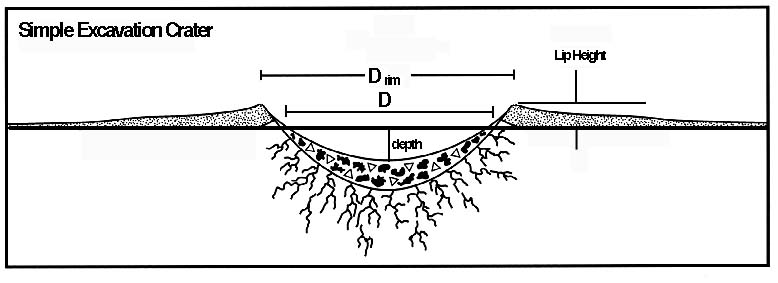
\includegraphics[scale=0.4]{simpleExcavationCrater-Holsapple.jpg}
	\caption{Example of a simple excavation crater, \url{http://keith.aa.washington.edu/craterdata/scaling/index.htm}.}\label{fig:simpleExcavationCrater-Holsapple}
\end{figure}

\subsubsection{Impact Event Parameters}
Impactor densities were chosen to be either cometary 1 g/cm$^3$, chondritic 3.4 g/cm$^3$, or iron-nickle 6 g/cm$^3$ with plausible impact velocities of 5-60 km/s. The diameter of the impactor was between 0.28 and 1.10 m with a mass between 33 and 702 kg. For this given range of impact velocities and densities, the kinetic energy of the impactor was between $6.4\times 10^9$ J and $6.0\times 10^{10}$ J.

\subsection{MEO Observations: Moser et al.\ 2014, ACM}
Here we summarize the findings from \cite{moser2014large}. They used both Gault's crater scaling law \citep{gault1974impact} and Holsapple's online calculator \citep{holsapple1993scaling} in their analysis.

\subsubsection{Correlation with Meteor Activity}
\cite{moser2014large} found correlation with the Virginid meteor shower complex (EVI/NVI) with an observed meteor shower on 17 March 2013 and the lunar impact that was seen by NASA MSFC. According to the \href{https://www.ta3.sk/IAUC22DB/MDC2007/Roje/pojedynczy_obiekt.php?kodstrumienia=00011&colecimy=1&kodmin=00001&kodmax=00569&sortowanie=0}{Meteor Data Center}, the eta Virginids, EVI, have a speed of 26.6 km/s to 34.2~km/s and the Northern March Virginids, NVI, have a speed of 23.0 km/s. However, given the cluster of five fireballs that were seen on 17 March 2013, the speed was $v_g = 25.6\pm 0.8$ km/s and matched closer to the EVI orbital elements. The Tisserand number was $3.1 \pm 0.2$, which is right on the line of being either cometary ($<3$) or asteroidal ($>3$). It was found that the lunar impact angle from the horizontal was $\theta_h = 56^\circ$ for a Virginid meteor.


\subsubsection{Impact Event Parameters}
Assuming a regolith density of $\rho_t = 1500$ kg/m$^3$, a porosity of 40\%, and cohesion strength of 0.1 Mpa, the impactor densities ranged from 1000 kg/m$^3$ to 3300 kg/m$^3$, the mass was between 11 kg and 66 kg, and the kinetic energy ranged from $3.6\times 10^9$~J to $2.2\times 10^{10}$ J. The duration of the impact was estimated to be 1.03 s with a nominal diameter of $22\pm 3$ cm, assuming $\rho_p = 3000$ kg/m$^3$.

\subsubsection{Luminous Efficiency}

From \cite{moser2014large}, if we assume the impactor was associated with the Virginids, the luminous efficiency $\eta_\lambda$ is in the range $7.5_{-2.5}^{+4.5} \times 10^{-4} < \eta_\lambda < 1.5_{-0.5}^{+0.8} \times 10^{-3}$, depending on the regolith density, $1500$ kg/m$^3 < \rho_t < 2100$ kg/m$^3$, and impactor density, $1000$ kg/m$^3 < \rho_t < 3300$ kg/m$^3$. This range of luminous efficiencies is consistent with \cite{bouley2012power} ($\eta_\lambda = 5\times 10^{-4}$) and \cite{moser2011luminous} ($\eta_\lambda = 1.3\times 10^{-3}$).

%\subsection{Summary for eta Virginids Impactor}
%%%%%%%%%%%%%%%%%%%%%%%%%%%%%%%%%%%%%%%%%%%%%%%%%%%%%%%%%%%%%%%%%%
%%%%%%%%%%%%%%%%%%%%%%%%%%%%%%%%%%%%%%%%%%%%%%%%%%%%%%%%%%%%%%%%%%
\section{Lunar Regolith Properties}



%%%%%%%%%%%%%%%%%%%%%%%%%%%%%%%%%%%%%%%%%%%%%%%%%%%%%%%%%%%%%%%%%%
%%%%%%%%%%%%%%%%%%%%%%%%%%%%%%%%%%%%%%%%%%%%%%%%%%%%%%%%%%%%%%%%%%
\section{Spheral Benchmark of 17 March 2013 Event}
\subsection{Getting Started and Running on Computer Clusters}
\subsubsection{Installing on MEO Cluster}

\lstinputlisting[language={}]{README-HowToCompileSpheralLocally.txt}

\subsubsection{Running on MEO Cluster}


\subsubsection{Running on LLNL Cluster}
The connection and login details described below is assumed to be on a \textsf{Windows} machine.

\begin{enumerate}
	\item Connect to VPN using \textsf{Cisco AnyConnect Secure Mobility Client}
	\begin{itemize}
		\item VPN name: \textsf{vpn.llnl.gov}
		\item Group name: \textsf{llnl.vpnc}
	\end{itemize}
	\item Login with \textsf{OUN} (\textsf{destefano2}) and \textsf{CZ PIN} + token \# (\textsf{RSA SecurID})
	\item SSH into LLNL server head node using \textsf{Putty}
	\begin{itemize}
		\item Host name: \textsf{rzgw.llnl.gov}
		\item Option: Connection $\rightarrow$ SSH $\rightarrow$ X11 $\rightarrow$ Enable X11 forwarding\footnote{Need to download either \textsf{VcXsrv} (works better), or \textsf{Xming}. In \textsf{VcXsrv}, which will be called \textsf{VLaunch} on the desktop, need to deselect \textbf{Native opengl} on the last tab.}
		\item Option: X display location $\rightarrow$ \textsf{localhost:0}
		\item Login: LC username (destefan)
		\item Password: RZ PIN + token \# (RZ)
	\end{itemize}
	\item SSH into RZ specific server
	\begin{itemize}
		\item \textsf{ssh -XY destefan@rztopaz}
		\item Password: RZ PIN + token \# (RZ)
	\end{itemize}
	\item Check current jobs for a user
	\begin{itemize}
		\item \textsf{squeue -u $<$username$>$}
		\item Add \textsf{- -start} to see begin ETA
	\end{itemize}
	\item Load Spheral module
	\begin{itemize}
		\item \textsf{ml Spheral/exp}
	\end{itemize}
	\item Debug Spheral Python script
	\begin{itemize}
		\item \textsf{srun -n $<$\# of CPUs, max 36 per node$>$ -p pdebug python -i $<$python\_script.py$>$}
		\item Add any variable definitions after the \textsf{python\_script.py}, such as \textsf{- -impactAngle=56}, \textsf{- -rImpactor=25.2}, etc. See the \textsf{halfSphere\_amdvX.py} file for more variable options.
	\end{itemize}
	\item Grab compute nodes for continuous debugging
	\begin{itemize}
		\item \textsf{mxterm $<$\# of nodes, max 8$>$ $<$\# of CPUs, =36$\times$\# of nodes, max 288$>$ $<$time, max 60 (minutes)$>$ -q pdebug}
		\item After nodes have been grabbed, do steps 6 and 7 as before 
	\end{itemize}
	\item Submit batch script
	\begin{itemize}
		\item \textsf{msub} $<$script.msub$>$
	\end{itemize}
	\item Check drive space quota
	\begin{itemize}
		\item \textsf{quota -v}
	\end{itemize}
\end{enumerate}


\subsection{Porosity $\phi_0$ Study}




\subsection{Max Strength $Y_m$ Study}


%%%%%%%%%%%%%%%%%%%%%%%%%%%%%%%%%%%%%%%%%%%%%%%%%%%%%%%%%%%%%%%%%%
%%%%%%%%%%%%%%%%%%%%%%%%%%%%%%%%%%%%%%%%%%%%%%%%%%%%%%%%%%%%%%%%%%
\section{Spheral Based Lunar Ejecta Modeling}
\label{sec:Spheral Based Lunar Ejecta Modeling}

%%%%%%%%%%%%%%%%%%%%%%%%%%%%%%%%%%%%%%%%%%%%%%%%%%%%%%%%%%%%%%%%%%
%%%%%%%%%%%%%%%%%%%%%%%%%%%%%%%%%%%%%%%%%%%%%%%%%%%%%%%%%%%%%%%%%%
\section{MEM3 Based Lunar Ejecta Modeling}
\label{sec:MEM3 Based Lunar Ejecta Modeling}
The \textsf{Meteoroid Engineering Model} (MEM) describes the sporadic meteoroid complex, or the background meteoroid environment, and does not include meteor showers. The impactor masses range from $1$ $\mu$g to $10$ g. Larger impactor masses must be dealt with differently \citep[e.g., see][]{neukum2001cratering, brown2002flux},\textit{ which we omit here for now}\footnote{At some point we will need to account for impactor masses larger than 10 g in order to understand the tail of the distribution in terms of the risk analysis.}. We use output from MEM in order to estimate the number of particles per area per year greater than a certain mass (or the particle flux mass spectrum) due to secondary ejecta from meteoroid impacts on the Moon. The risk due to impacts on the Moon is driven by secondary ejecta and not the primary meteoroid flux.

We begin by first describing the algorithm at which we plan to use to compute the particle flux mass spectrum at a given point on the Moon. In essence, the algorithm is based on the reverse Monte-Carlo idea. We then go into detail about how to compute each step of the algorithm, either borrowing from the literature or making our own derivations.

\subsection{Algorithm}
\begin{enumerate}
	\item For a given location on the Moon, compute the particle flux mass spectrum
	\item For each source location
	\begin{itemize}
		\item Defines the distance $D$ from the source required to compute the ejecta velocity $v = v(D,\gamma)$.
	\end{itemize}
	\item For each ejecta angle $\gamma$
	\begin{itemize}
		\item Completely defines the ejecta velocity $v = v(D,\gamma)$
	\end{itemize}
	\item For each meteoroid impact angle $\alpha$ (from MEM output)
	\begin{itemize}
		\item At the moment, we will sum over the azimuthal angle and assume isotropic azimuthal seconday ejecta (this is not the case for impact angles less than 30$^\circ$ from the horizon).
	\end{itemize}
	\item For each meteoroid impact speed $U$
	\item For each impactor density $\delta$
	\begin{itemize}
		\item We only need to compute this once for each target material, and can factor out as a constant. The density is given as an output in MEM.
	\end{itemize}
	\item For each impactor mass $m_p$
	\begin{itemize}
		\item We can integrate this out. At first glance, we will get a list of hypergeometric functions, but we only need to evaluate these once and factor out as a constant. The mass distribution is given in MEM Eq.\ (2.1).
	\end{itemize}
	\item For each ejecta particle size $m_e$
	\begin{itemize}
		\item  We can integrate the particle size distribution, but we will need to keep track of each mass size $m_e$.
	\end{itemize}
\end{enumerate}


%%%%%%%%%%%%%%%%%%%%%%%%%%%%%%%%%%%%%%%%%%%%%%%%%%%%%%%%%%%%%%%%%%
\subsection{Regolith Size Distribution}
For relatively small impact sizes (craters $<30-50$ m), we can generally assume the secondary ejecta follows that of the original regolith. The cumulative distribution function (CDF) of the particle sizes can be fit to many observations, as shown in Figure~\ref{fig:Carrier2003_Fig1_particle-size-distribution}.

\begin{figure}[h!]
	\centering
	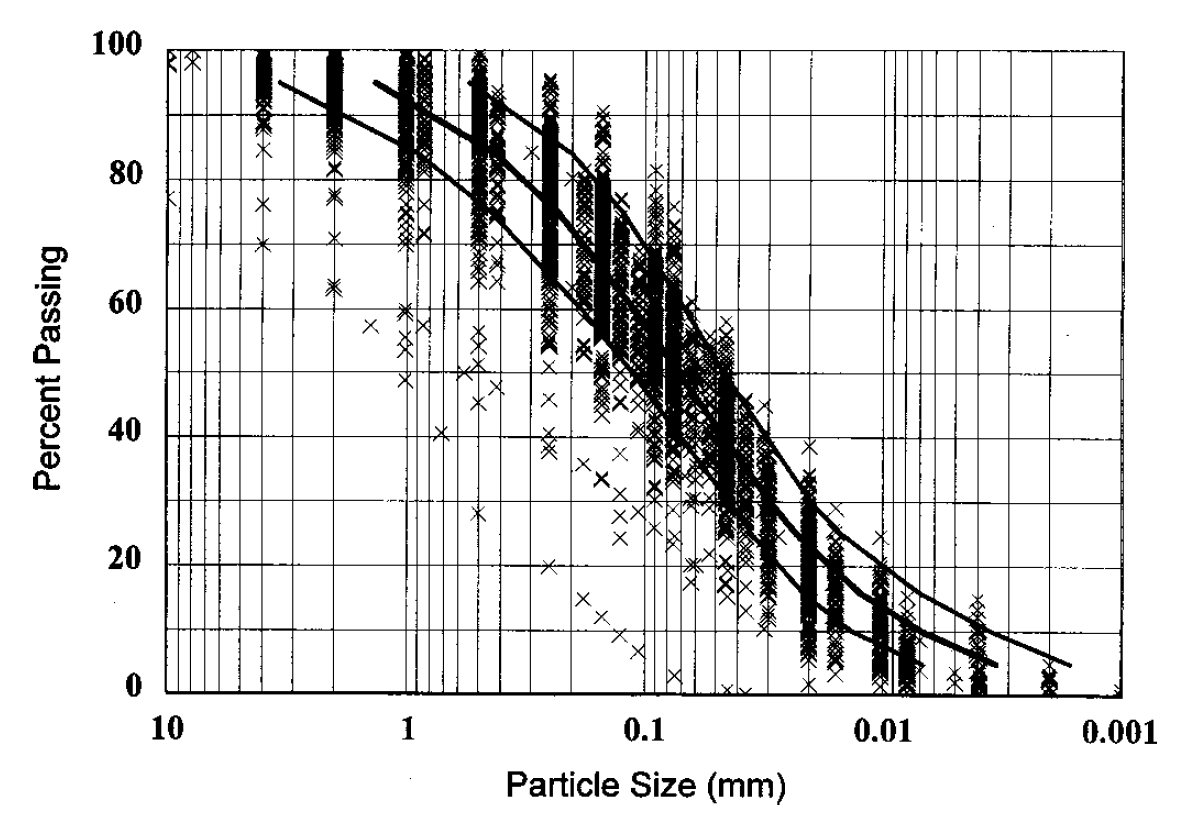
\includegraphics[scale=0.4]{Carrier2003_Fig1_particle-size-distribution.PNG}
	\caption{Geotechnical particle size distribution: midlle curve showing the average distribution; left-hand and right-hand curves showing $\pm$1 standard deviation \citep{carrier2003particle}.}\label{fig:Carrier2003_Fig1_particle-size-distribution}
\end{figure}

In order to parametrize the CDF from Figure \ref{fig:Carrier2003_Fig1_particle-size-distribution}, we make a fit to the model equation
\begin{equation}\label{eq:particle-CDF}
C_{moon} = 1 - \exp\left(\frac{-1}{ax^b+cx^d}\right),
\end{equation}
which is an exponential distribution with two scales defined by $a$ and $c$, with $x$ in units of mm. In \textsf{SciDAVis}, we make the fit with the x-axis on a logarithmic scale to give equal weight to both small and large scaled particles. The results for the curve fit are shown in Figure \ref{fig:Fit-to-CDF}. We found that a simple exponential distribution with a single scale was insufficient, hence the reason we opted for a two-scaled exponential distribution.

\begin{figure}[h!]
	\centering
	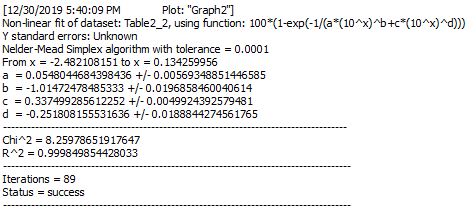
\includegraphics[scale=1]{Fit-to-CDF.PNG}
	\caption{Non-linear fit of Figure \ref{fig:Carrier2003_Fig1_particle-size-distribution} (the average distribution) with Eq.\ \ref{eq:particle-CDF} in \textsf{SciDAVis}, giving the constants for $a$, $b$, $c$, and $d$.}\label{fig:Fit-to-CDF}
\end{figure}

To compute the probability distribution function (PDF), we can simply take the derivative of the CDF with respect to $x$, which results in the following equation:
\begin{equation}
P_{moon} = -A\frac{abx^{b-1}+cdx^{d-1}}{(ax^b+cx^d)^2}\exp\left(\frac{-1}{ax^b+cx^d}\right),
\end{equation}
where $A$ is the normalization constant. In theory, this should be equal to 1, but since we are not taking our particle size from 0 to infinity, we need to compute the value of $A$. If we assume the particle size can range from $0.001$ mm to $10$ mm, then $A = 1.02218$.

Since our goal is to compute the particle flux mass spectrum, we need to \textit{count} the number of particles from the PDF that make up the mass of $M$ from Eq.\ \ref{eq:HH11_mass-ejected1}. We first need to know the total volume per complete PDF, which is given by
\begin{equation}\label{eq:VPmoon}
V_{P_{moon}}(x_{min}) = \frac{4}{3}\pi \int_{x_{min}}^{x_{max}}dx x^3 P_{moon}(x),
\end{equation}
where $x_{min} = 0.001$ mm and $x_{max} = 10$ mm. An exact analytic solution of Eq.\ \ref{eq:VPmoon} is quite difficult, but we notice that the integrand $x^3 P_{moon}(x)$ very closely resembles a linear equation within the desired range, see Figure \ref{fig:Fit-to-x3PDF}.

\begin{figure}[h!]
	\centering
	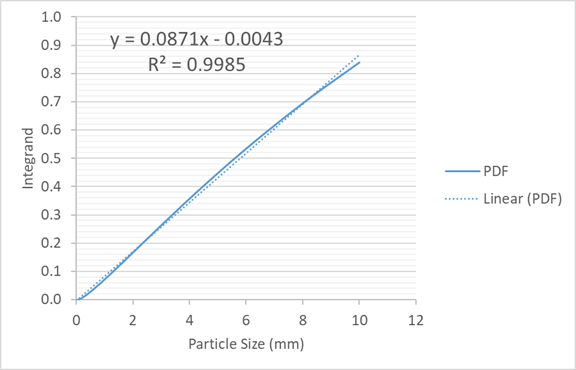
\includegraphics[scale=0.7]{Fit-to-x3PDF.png}
	\caption{Linear fit to the integrand $x^3 P_{moon}(x)$.}\label{fig:Fit-to-x3PDF}
\end{figure}

Therefore, we make the approximation
\begin{equation}
x^3 P_{moon}(x) \sim p_0 x + p_1,
\end{equation}
where $p_0 = 1/11.48$ and $p_1 = 1/232.6$. The total volume of particles with mass greater than $m_{0} = \frac{4}{3}\pi\rho x_{0}^3$ is given by
\begin{equation}\label{eq:VPmoon2}
V_{P_{moon}}(x_{0}) = \frac{4}{3}\pi \left[\frac{1}{22.96}\left(x_{max}^2 - x_{0}^2\right) - \frac{1}{232.6}\left(x_{max} - x_{0}\right)\right],
\end{equation}
where $V_{P_{moon}}(x_{min}) = 18.06377$ mm$^3$. Given the density of the regolith $\rho$, we can then compute the total mass of the particles from the PDF.

%%%%%%%%%%%%%%%%%%%%%%%%%%%%%%%%%%%%%%%%%%%%%%%%%%%%%%%%%%%%%%%%%%
\subsection{Ejected Mass from an Impactor}
From \cite{housen2011ejecta}, we can compute the mass ejected faster than $v$ in terms of impactor properties, given by
\begin{eqnarray}\label{eq:HH11_mass-ejected1}
M(v; \rho; m, \delta, U, \alpha) = M(>v) = C_4 m\left[\frac{v}{U\Theta(\alpha)}\left(\frac{\rho}{\delta}\right)^{\frac{3\nu-1}{3\mu}}\right]^{-3\mu},
\end{eqnarray}
where
\begin{itemize}
	\item $v$: secondary ejecta speed,
	\item $\rho$: target density,
	\item $m$: projectile mass,
	\item $\delta$: projectile density,
	\item $U$: projectile speed,
	\item $\alpha$: projectile impact angle (from horizon),
\end{itemize}
and
\begin{eqnarray}
C_4 = \frac{3k}{4\pi}C_1^{3\mu},
\end{eqnarray}
where the constants $k$, $C_1$, $\nu$, and $\mu$ depend on the specific material properties, see Table 3 of \cite{housen2011ejecta}. The impact angle modification equation $\Theta(\alpha)$ can be chosen to be
\begin{equation}
\Theta(\alpha) = \begin{cases}
1\\
\sin\alpha\\
\sin(\sqrt{\alpha_0^2 + \alpha^2}),\text{  } \alpha_0 \sim 5^\circ-15^\circ.
\end{cases}
\end{equation}

For the ejected mass that is in a given velocity range, we can define $\Delta M(v_2, v_1)$ as
\begin{equation}\label{eq:delta_M}
\Delta M(v_2, v_1) = M(>v_2) - M(>v_1).
\end{equation}

\subsection{Ejecta Mass Distribution Function}

The mass ejected from the crater, $M(>v)$, from Eq.\ \eqref{eq:HH11_mass-ejected1}, is the total mass ejected from an impact at velocities greater than $v$. However, we would like to know how this ejecta is distributed in speed and solid angle so we can map the ejecta to a particular surface location on the Moon. We can then set Eq.\ \eqref{eq:HH11_mass-ejected1} in terms of the integral over the distribution functions of speed and solid angle as
\begin{equation}
M(>v) = \int_{v}^{\infty}\int_{0}^{2\pi}\int_{0}^{\pi/2}\sin\alpha d\alpha d\beta dv' F(\alpha)G(\beta)H(v'),
\end{equation} 
where $\alpha$ is the zenith angle, $\beta$ is the azimuth angle, and $v$ is the ejecta speed. Just to note, at the secondary impact location, the zenith angle will be the same as the ejected zenith angle. However, the azimuth angle (or bearing) will be modified due to travel across the spherical surface, see Section \ref{ssec:Distance_and_Bearing}.



\subsubsection{Zenith Distribution Function}
\label{sssec:ZenithDistributionFunction}


For the angular dependent terms $F(\alpha)$ and $G(\beta)$, they technically should depend on speed as well as particle size \citep[e.g.,][]{rival1999modeling}. For simplicity, we will assume the angular distribution is independent of speed and particle size but will be dependent on impact zenith and azimuth angle with respect to the bearing.

Adopting the zenith and azimuth distributions from \cite{rival1999modeling}, we have the following equations:
The zenith distribution is given by
\begin{equation}\label{eq:Rival_zenith-dist}
F(\alpha) = \frac{1}{\sigma\sqrt{2\pi}}\exp\left[-\frac{(\alpha-\alpha_{max})^2}{2\sigma^2}\right],
\end{equation}
where $\alpha_{max}$ is defined as
\begin{equation}
\alpha_{max} = 
\begin{cases}
\frac{\alpha_{max60}-\alpha_{max0}}{\pi/3}\alpha_i + \alpha_{max0}\text{  for $\alpha_i\le \pi/3 = 60^\circ$}\\
\alpha_{max60}\text{  for $\alpha_i > \pi/3 = 60^\circ$}
\end{cases},
\end{equation}
for $\alpha_i$ the impact zenith angle, and \citep[see][]{ESABASE2_DebrisRelease10.0}
\begin{align}
\alpha_{max0} &= \frac{\pi}{6} = 30^\circ,\\
\alpha_{max60} &= \frac{4\pi}{9} = 80^\circ,\\
\sigma &= \frac{\pi}{60} = 3^\circ,
\end{align}
where the peak ejecta angle is shifted from $30^\circ$ of zenith for a normal impact to $80^\circ$ of zenith for oblique impacts ($>60^\circ$).

\paragraph{Alternative Zenith Distribution:}
To complete the integral over the zenith distribution, namely
\begin{equation}\label{eq:zenith_integral}
\int_{\alpha_0(v)}^{\alpha_1(v)}d\alpha\sin\alpha F(\alpha),
\end{equation}
we need to choose a distribution function for $F(\alpha)$ to allow for analytic solutions. We will therefore look for an alternate distribution from Eq.\ \eqref{eq:Rival_zenith-dist}, given by the form
\begin{equation}
F(\alpha) = (1-\cos\alpha)^{1/a}\cos^a\alpha,
\end{equation}
where the exponent $a$ can be defined in terms of the peak angle $\alpha_{max}$ as
\begin{equation}
a = \frac{\cos\alpha_{max}}{1-\cos\alpha_{max}},
\end{equation}
such that $F'(\alpha_{max}) = 0$ and $F''(\alpha_{max}) < 0$.

In order to compare with experiments for the peak angle $\alpha_{max}$, we can use Figure~18 of \cite{gault1978experimental} as a proxy to our model of $\alpha_{max}$, as a function of the azimuth angle. Using a third order polynomial for both fits to the upstream and downstream angles given in Table \ref{tab:upstream_downstream_angles}, we arrive at
\begin{align}
\alpha_{max}(\beta - \beta_i = \pi) &= 0.0003\alpha_i^3 - 0.036\alpha_i^2 + 1.5206\alpha_i + 20,\\
\alpha_{max}(\beta - \beta_i = 0) &= -0.00042\alpha_i^3 + 0.0236\alpha_i^2 + 0.129\alpha_i + 20,
\end{align}
in units of degrees, where $\beta_i$ is the impact azimuth angle, $\beta$ is the ejecta azimuth angle, and $\alpha_i$ is the impact zenith angle. For other values of $\beta - \beta_i$, we can write a complete function as
\begin{equation}
\alpha_{max}(\beta) = \alpha_{max}(\beta - \beta_i = \pi)\cdot \sin^2\left(\frac{\beta - \beta_i}{2}\right)
+ \alpha_{max}(\beta - \beta_i = 0)\cdot \cos^2\left(\frac{\beta - \beta_i}{2}\right)
\end{equation}

\begin{table}[h]\centering
	\caption{Cone angles of upstream and downstream of impact derived from Figure 18 of \cite{gault1978experimental}.}\label{tab:upstream_downstream_angles}
	\begin{tabular}{|c | c | c |}\hline
		Impact Zenith Angle & Upstream Zenith Angle & Downstream Zenith Angle\\\hline
		0	&20	&20\\\hline
		15	&24	&35\\\hline
		30	&35	&45\\\hline
		45	&28	&40\\\hline
		60	&13	&54\\\hline
		75	&-35	&66\\\hline		
	\end{tabular}
\end{table}
Using Table \ref{tab:upstream_downstream_angles} as a fit for the peak angle $\alpha_{max}$ is an approximation since the tabular data is only for a specific snapshot of the ejecta at a side view, $90^\circ$ from the impact direction. The zenith distribution should also be a function of the ejecta speed, but we do not make this assumption for the sake of simplicity. According to this model, starting around $60^\circ - 70^\circ$, there is a region of exclusion for a part of the zenith distribution upstream of the impact, see Figure \ref{fig:ExlusionRange_vs_ImpactAngle}.


\begin{figure}[h!]
	\centering
	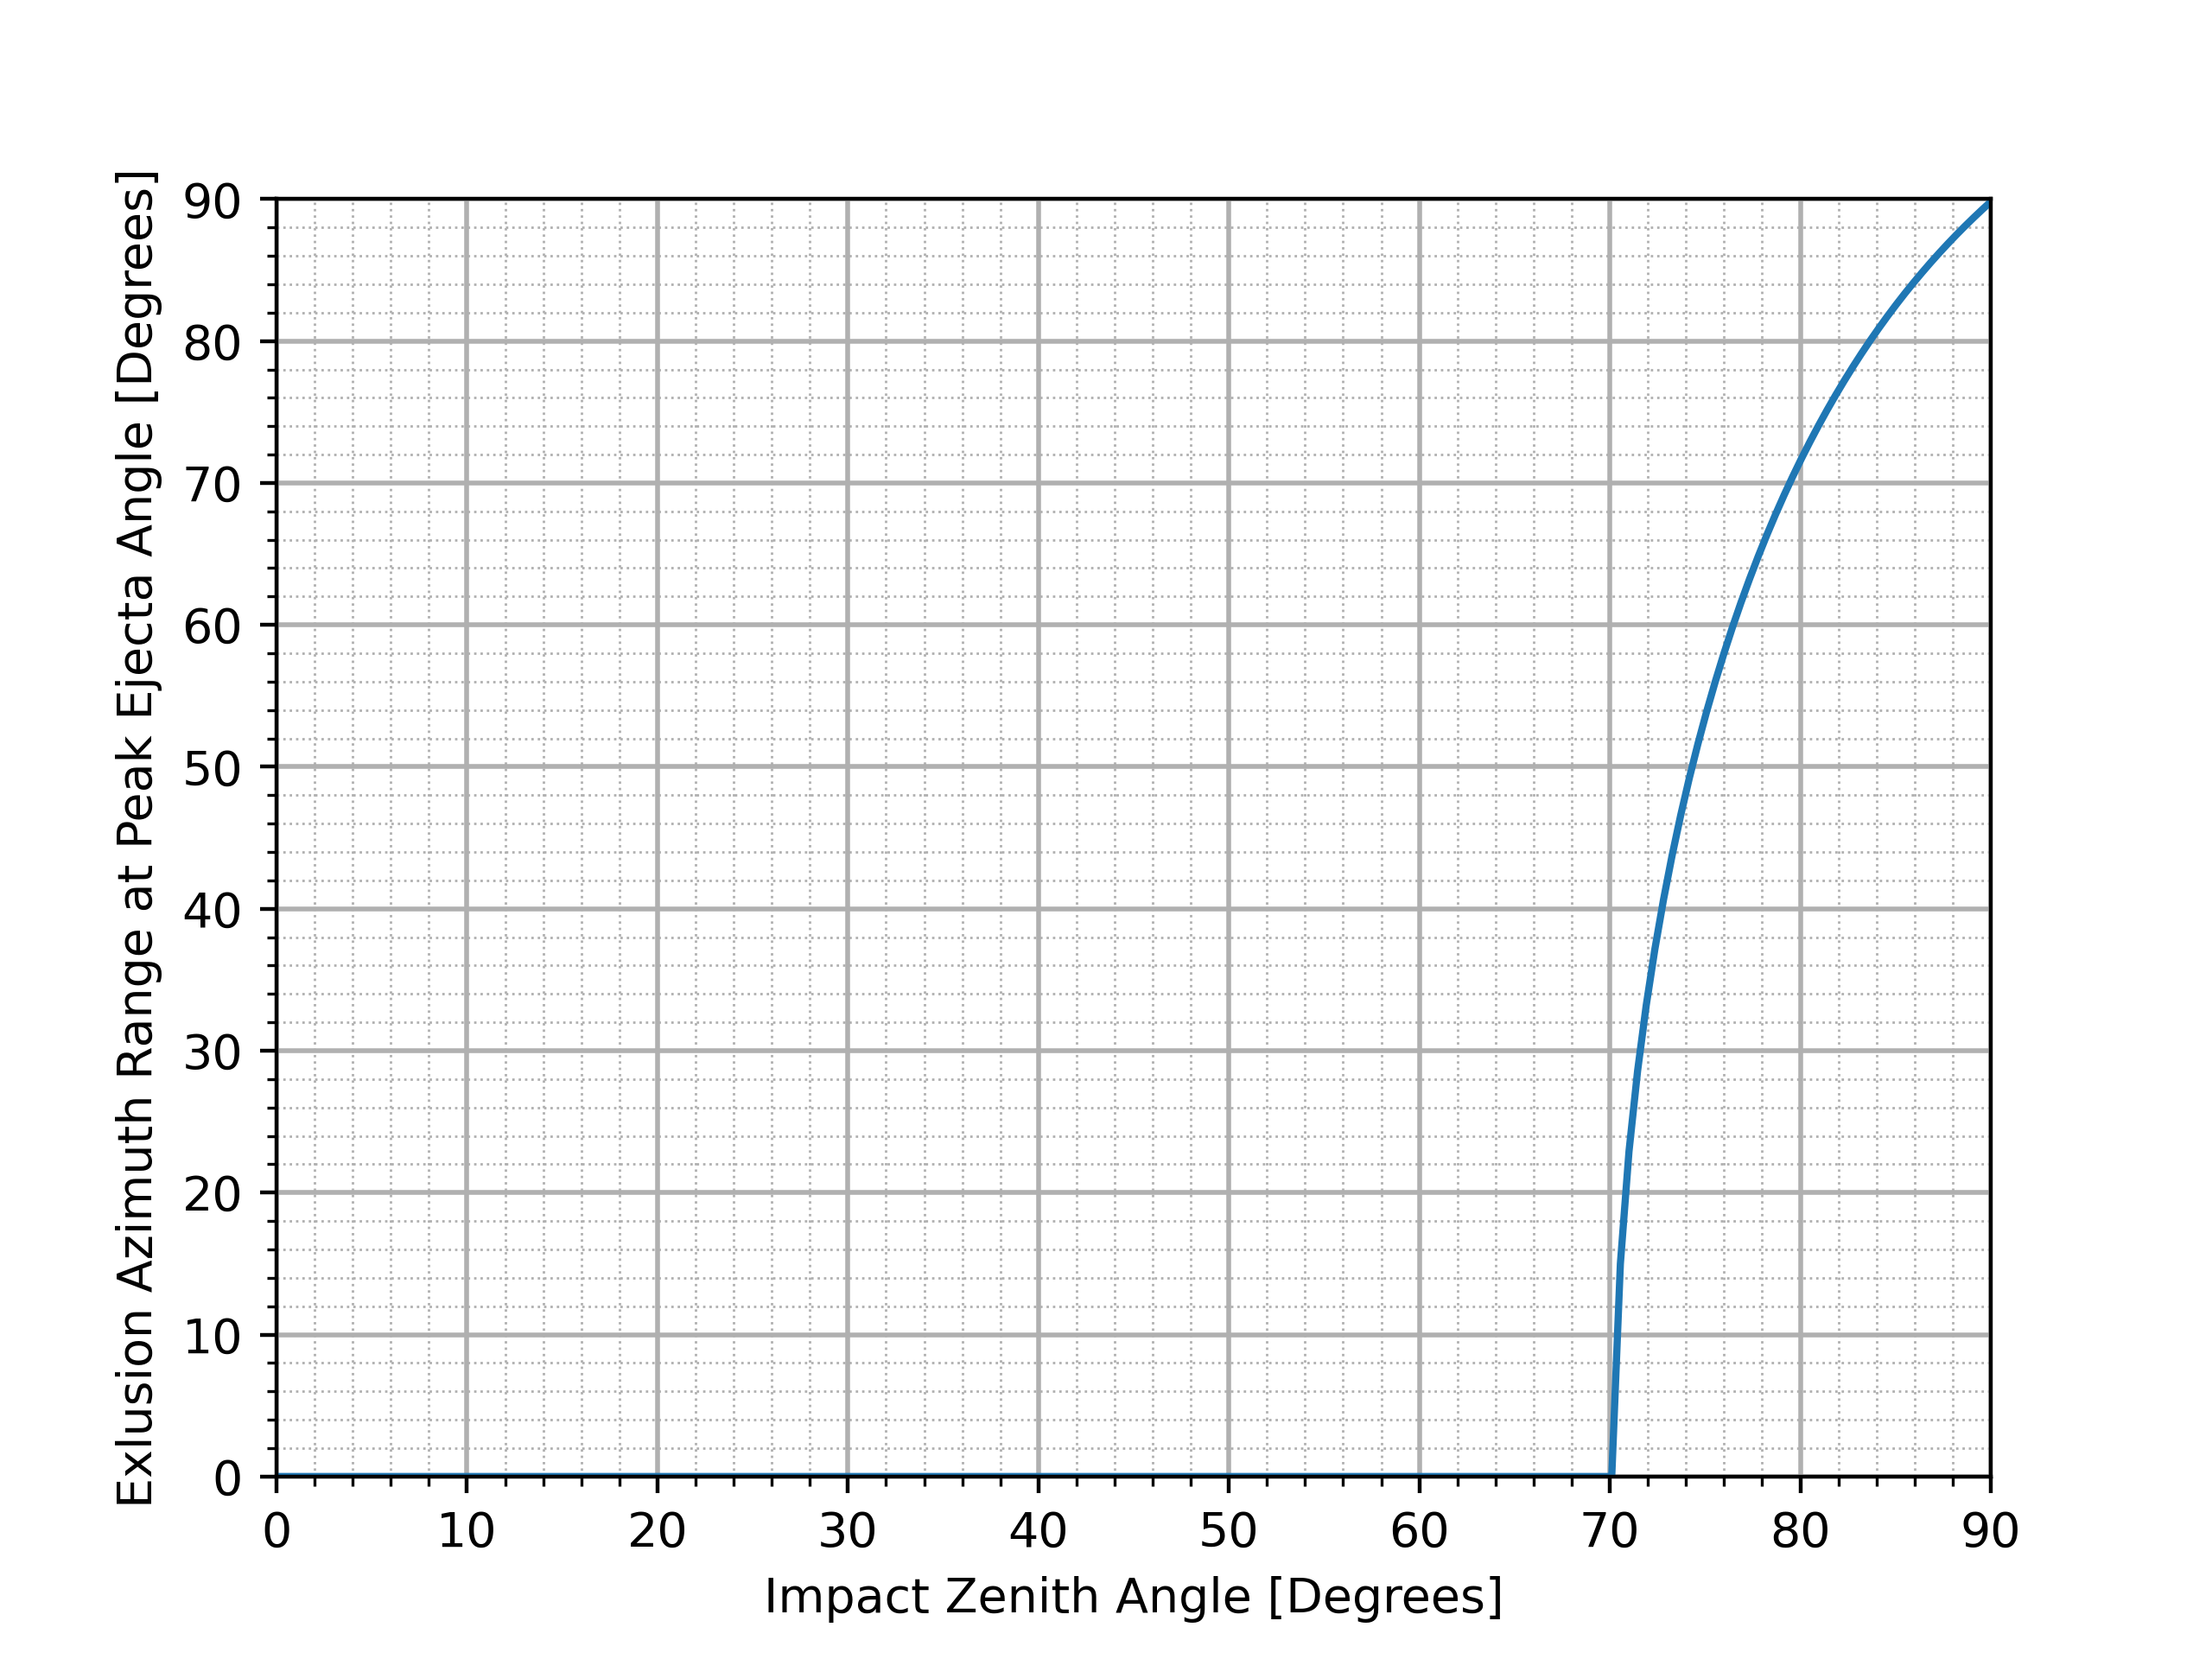
\includegraphics[scale=0.65]{ExlusionRange_vs_ImpactAngle.png}
	\caption{For larger impact angles that are more grazing to the surface, the zenith and azimuth ejecta distributions become asymmetric. Starting at $70^\circ$, the peak ejecta angle $\alpha_{max}$ becomes negative in an exclusion range, as shown in the figure. This means that the $-\alpha_{max}\to\alpha_{max}$ and $\beta-\beta_i\to \beta-\beta_i +\pi$. In this model, for impact angles near $90^\circ$, most of the ejecta is concentrated in the downstream direction.}\label{fig:ExlusionRange_vs_ImpactAngle}
\end{figure}

%
%\begin{tikzpicture}\centering
%\begin{axis}[
%	xlabel = Impact Zenith Angle,
%	ylabel = Exlusion Azimuth Range at Peak Ejecta Angle
%]
%\addplot coordinates {
%	( 338.1, 266.45 )
%	( 169.1, 143.43 )
%	( 84.5, 64.80 )
%	( 42.3, 34.19 )
%	( 21.1, 9.47 )
%};
%\end{axis}
%\end{tikzpicture}

Next, we can do a variable substitution (chosen so the domain of the zenith angle to the new variable goes from $\alpha\in [0,\pi/2]$ to $x\in [0,1]$)
\begin{align}
1-x &= \cos\alpha,\\
dx &= \sin\alpha d\alpha,
\end{align}
so that Eq.\ \eqref{eq:zenith_integral} becomes
\begin{equation}\label{eq:zenith_integral2}
\int_{x_0(v)}^{x_1(v)}dx x^{1/a}(1-x)^a,
\end{equation}
where the equations $x_0(v)$ and $x_1(v)$ are a linear function of $v$ and an implicit function of the distances $D_0$ and $D_1$, respectively. The integral in Eq.\ \eqref{eq:zenith_integral2} is the incomplete beta function
\begin{equation}\label{eq:zenith_integral3}
\int_{x_0(v)}^{x_1(v)}dx x^{1/a}(1-x)^a
= \beta(x_1(v); 1/a+1, a+1) - \beta(x_0(v); 1/a+1, a+1).
\end{equation}
Note that the normalization term for $\alpha\in [0, \pi/2]$ is given by
\begin{equation}
\int_{0}^{\pi/2}d\alpha\sin\alpha F(\alpha) = 
\beta(1/a+1, a+1) = \frac{\Gamma(1/a+1)\Gamma(a+1)}{\Gamma(a+1/a+2)},
\end{equation}
which includes ejecta at speeds greater than the escape speed.

For small differences in $D_0$ and $D_1$, we can roughly assume small differences\footnote{If $\Delta x$ is not small, then we can partition the $x$ range into smaller pieces so that $\Delta x$ is small, which will be the case in almost all circumstances.} in $x_0(v)$ and $x_1(v)$ so that we can write Eq.\ \eqref{eq:zenith_integral3} in terms of a derivative, where we evaluate the derivative at the midpoint
\begin{align}
&\beta(x_1(v); 1/a+1, a+1) - \beta(x_0(v); 1/a+1, a+1)\nonumber\\
= &\frac{\beta(x_0(v) +\Delta x; 1/a+1, a+1) - \beta(x_0(v); 1/a+1, a+1)}{\Delta x}\Delta x\nonumber\\
\approx & \Delta x\frac{d}{d(x_0(v))}\beta(x_0(v); 1/a+1, a+1)\Bigr|_{x_0(v)\to x_0(v) +\Delta x/2}\nonumber\\
=& \Delta x\left[1-x_0(v)\right]^a x_0^{1/a}(v)\Bigr|_{x_0(v)\to x_0(v) +\Delta x/2}\nonumber\\
=&\Delta x(v)\left[1-\frac{x_0(v)+x_1(v)}{2}\right]^a \left[\frac{x_0(v)+x_1(v)}{2}\right]^{1/a},
\end{align}
where $\Delta x(v) = x_1(v) - x_0(v)$, and (note, the $v$'s are normalized by $v_{esc}$, emitted for clarity)
\begin{align}
x_0(v) &= m_0 v + b_0,\\
x_1(v) &= m_1 v + b_1,\\
\Delta x(v) &= (m_1-m_0)v + b_1 - b_0.
\end{align}
The coefficients $m_0, m_1$ and $b_0, b_1$ are implicit functions of the distances $D_0, D_1$. For the $j-$th distance $D_j$ and the $i-$th speed $v_i$, the $m$ and $b$ coefficients can be written as
\begin{align}
m_{j,i}^{\pm} &= \frac{v_{i+1}-v_i}{x_{j,i+1}^{\pm}-x_{j,i}^{\pm}},\\
b_{j,i}^{\pm} &= v_i - m_{j,i}^{\pm}\cdot x_{j,i}^{\pm},
\end{align}
where
%\begin{align}
%x_{j,i}^{\pm} &= 1 - \cos\alpha_{j,i}^{\pm}, \\
%\cos\alpha_{j,i}^{\pm} &= \frac{\cot\alpha_{j,i}^{\pm}}{\sqrt{1+ \cot^2\alpha_{j,i}^{\pm}}},
%\end{align}
%for (using Eq.\ \eqref{eq:gammaVs_V_D})
%\begin{equation}
%\cot\alpha_{j,i}^{\pm} = v_i^2\cot\left(\frac{D_j}{2r_m}\right) \pm \sqrt{v_i^4\cot^2\left(\frac{D_j}{2r_m}\right) +2v_i^2-1 }.
%\end{equation}

\begin{equation}
x_{j,i}^{\pm} = 1 - \cos\alpha_{j,i}^{\pm},
\end{equation}
for
\begin{equation}
\cos^2\alpha_{j,i}^{\pm} = \frac{v_i^2+\tan^2\left(\frac{D_j}{2r_m}\right)(2v_i^2-1) \pm \sqrt{v_i^4 + \tan^2\left(\frac{D_j}{2r_m}\right)(2v_i^2-1)}}{2v_i^2\left(1 + \tan^2\left(\frac{D_j}{2r_m}\right)\right) },
\end{equation}
taking the positive root, $\cos\alpha_{j,i}^{\pm} = +\sqrt{\cos^2\alpha_{j,i}^{\pm}}$, since $\alpha\in [0, \pi/2]$. Other useful transformed equations are
\begin{equation}
\tan\left(\frac{D_j}{2r_m}\right) = \frac{2v_i^2(1-x_{j,i}^{\pm})\sqrt{x_{j,i}^{\pm}(2-x_{j,i}^{\pm})}}{1-2v_i^2x_{j,i}^{\pm}(2-x_{j,i}^{\pm})},
\end{equation}
from Eq.\ \eqref{eq:ejecta_distance}, and
\begin{equation}
v_i = \frac{1}{\sqrt{2(1-x_{j,i}^{\pm})\sqrt{x_{j,i}^{\pm}(2-x_{j,i}^{\pm})}\cot\left(\frac{D_j}{2r_m}\right) + 2x_{j,i}^{\pm}(2-x_{j,i}^{\pm})}},
\end{equation}
from Eq.\ \eqref{eq:speed_asof_distance_angle}. Solving for $x_{j,i}^{\pm}$ in either equation, we can now write $x$ explicitly in terms of the distance $D$ and ejecta speed $v$ as
\begin{equation}
x_{j,i}^{\pm} = 1 - \sqrt{\frac{v_i^2 + \tan^2\left(\frac{D_j}{2r_m}\right)(2v_i^2-1) \pm \sqrt{v_i^4 + \tan^2\left(\frac{D_j}{2r_m}\right)(2v_i^2-1)}}{2v_i^2\left[1+\tan^2\left(\frac{D_j}{2r_m}\right)\right]}}.
\end{equation}

For a given distance, the domain of $x$ is given by (for $v$ up to 1)
\begin{equation}\label{eq:x_domain} %\sqrt{\frac{1+\cos\left(\frac{D_j}{2r_m}\right)}{2}}
x_{j,i}^{\pm} \in \left(1 - \cos\left(\frac{D_j}{4r_m}\right),
1 \right),
\end{equation}
and the domain of $v$ is given by
\begin{equation}\label{eq:v_domain}
v_i \in
\begin{cases}
\left(\left[1 + \left|\cos\left(\frac{D_j}{2r_m}\right)\right|\cot\left(\frac{D_j}{2r_m}\right) + \sin\left(\frac{D_j}{2r_m}\right) \right]^{-1/2}, 1\right) \text{  for $D_j < \pi r_m$}\\
\left(\frac{\sqrt{2}}{2}, 1\right) \text{  for $D_j \ge \pi r_m$}
\end{cases}
\end{equation}
where the value of $x_{j,i}^{\pm}$ at the minimum of $v_i$ is
\begin{equation}
x_{j,i}^{\pm} = 1-\sqrt{\frac{1-\sin\left(\frac{D_j}{2r_m}\right)}{2}}
\end{equation}
The two domains in Eqs.\ \eqref{eq:x_domain} and \eqref{eq:v_domain} define the region of interest, and allow for the integration to begin at the correct outermost boundary lines.

There are three regions of the zenith angle-space, and hence the $x$-space, where we have:
\begin{enumerate}[label=Region \Roman*:]
	\item For all valid distances $D_j$ and $D_{j+1}$, use $m_{j,i}^{+}$, $b_{j,i}^{+}$, $m_{j+1,i}^{+}$ and $b_{j+1,i}^{+}$
	\item For $D_j < \pi r_m$ and all $D_{j+1}$, use $m_{j,i}^{-}$, $b_{j,i}^{-}$, $m_{j+1,i}^{+}$ and $b_{j+1,i}^{+}$
	\item For $D_j < \pi r_m$ and $D_{j+1} < \pi r_m$, use $m_{j,i}^{-}$, $b_{j,i}^{-}$, $m_{j+1,i}^{-}$ and $b_{j+1,i}^{-}$
\end{enumerate}



\subsubsection{Azimuth Distribution Function}
\label{sssec:AzimuthDistributionFunction}

The azimuth distribution shown below is given by \citep{rival1999modeling}
\begin{equation}\label{eq:azm_rival_mandeville}
G(\beta) =
\begin{cases}
\frac{1}{2\pi}\left[\frac{3\alpha_i}{2\pi - 3\alpha_i}\cos(\beta-\beta_i)+1\right] \text{  for $\alpha_i\le \pi/3 = 60^\circ$}\\
\frac{1}{\sigma'\sqrt{2\pi}}\exp\left[-\frac{(\beta-\beta_i)^2}{2\sigma'^2}\right]
\text{  for $\alpha_i > \pi/3 = 60^\circ$}
\end{cases},
\end{equation}
where
\begin{equation}
\sigma' = \frac{\pi}{36} = 5^\circ, 
\end{equation}
for $\beta_i$ the impact azimuth angle + $\pi$.\\

\paragraph{Alternative Azimuth Distribution:}
The piece-wise function defined in Equation \eqref{eq:azm_rival_mandeville} for the azimuth distribution is correctly normalized for impact zenith angles $\alpha_i \le 60^\circ$, however for angles greater than $60^\circ$, the function is not continuous across the boundary $\beta = 2\pi \to 0$. We would also like a continuous function across the piece-wise boundary as well.

Our proposed azimuth distribution is as follow. We will use the $\alpha_i \le 60^\circ$ functional form in Equation \eqref{eq:azm_rival_mandeville}, but we will have a different large-angle expression. The new azimuth distribution is defined as
\begin{equation}
G(\beta) =
\begin{cases}
\frac{1}{2\pi}\left[\frac{3\alpha_i}{2\pi - 3\alpha_i}\cos(\beta-\beta_i)+1\right] \text{  for $\alpha_i\le \pi/3 = 60^\circ$}\\
\frac{\Gamma(b+1)}{2\sqrt{\pi}\Gamma(b+1/2)}\left[\cos^2\left(\frac{\beta-\beta_i}{2}\right)\right]^{b}
\text{  for $\alpha_i > \pi/3 = 60^\circ$}
\end{cases},
\end{equation}
where
\begin{equation}
b = 1 + \left[20\left(\frac{3\alpha_i}{\pi}-1\right)\right]^2.
\end{equation}
Notice we already have normalized both piece-wise expressions.

For $\alpha_i > \pi/3 = 60^\circ$, in order to integrate over a small azimuth range $\beta\in(\beta_0, \beta_1)$
\begin{equation}
\frac{\Gamma(b+1)}{2\sqrt{\pi}\Gamma(b+1/2)}\int_{\beta_0}^{\beta_1}d\beta \left[\cos^2\left(\frac{\beta-\beta_i}{2}\right)\right]^{b},
\end{equation}
we can take the Taylor expansion of the integrand around the midpoint $\beta = \beta_{avg} = \frac{\beta_0+\beta_1}{2}$, such that
\begin{align}
&\frac{\Gamma(b+1)}{2\sqrt{\pi}\Gamma(b+1/2)}\int_{\beta_0}^{\beta_1}d\beta \left[\cos^2\left(\frac{\beta-\beta_i}{2}\right)\right]^{b}\nonumber\\
\sim &\int_{\beta_0}^{\beta_1}d\beta \left[G(\beta_{avg}) + G'(\beta_{avg})(\beta-\beta_{avg}) + G''(\beta_{avg})(\beta-\beta_{avg})^2 + \dots\right].
\end{align}
We notice that all odd powers of $(\beta-\beta_{avg})$ integrate to zero, so if we keep the second order expansion term $G''$, then our error will be of order\footnote{We gain an extra order from the integration range itself.} $\Delta\beta^5 = (\beta_1-\beta_0)^5$. Therefore, the integral becomes
\begin{align}
&A\int_{\beta_0}^{\beta_1}d\beta \left[\cos^2\left(\frac{\beta-\beta_i}{2}\right)\right]^{b}\nonumber\\
\sim & A\Delta\beta
\left[\cos^2\left(\frac{\beta_{avg}-\beta_i}{2}\right)\right]^{b}
\left[1 + \frac{b}{12}\Delta\beta^2\left[\frac{b\sin^2\left(\frac{\beta_{avg}-\beta_i}{2}\right) - \frac{1}{2}}{\cos^2\left(\frac{\beta_{avg}-\beta_i}{2}\right)}\right]\right],
\end{align}
where $A$ is the normalization factor we had before
\begin{equation}
A = \frac{\Gamma(b+1)}{2\sqrt{\pi}\Gamma(b+1/2)}.
\end{equation}\\

For $\alpha_i\le \pi/3 = 60^\circ$, integrating over a small range $\Delta\beta = \beta_1-\beta_0$, the integral is given by
\begin{align}
&\frac{1}{2\pi}\int_{\beta_0}^{\beta_1}d\beta \left[\frac{3\alpha_i}{2\pi-3\alpha_i}\cos(\beta-\beta_i)+1\right]\nonumber\\
=& \frac{1}{2\pi}\left[\Delta\beta + \frac{3\alpha_i}{2\pi-3\alpha_i}\left[\sin(\beta_1-\beta_i) - \sin(\beta_0-\beta_i)\right]\right].
\end{align}


\subsubsection{Speed Distribution Function}

The speed distribution $H(v')$ is defined by
\begin{equation}
\int_{v}^{\infty}dv'H(v') = v^{-3\mu},
\end{equation}
which is the speed dependent term of Eq.\ \eqref{eq:HH11_mass-ejected1}. We can then solve the speed distribution explicitly as
\begin{equation}
H(v) = 3\mu v^{-(3\mu+1)}.
\end{equation}

To integrate over the velocity distribution, we must take the results from Section~\ref{sssec:ZenithDistributionFunction} on the zenith distribution function and combine them with the above integral, giving

\begin{align}
&3\mu\int_{v_0}^{v_1}dv v^{-(3\mu+1)}\Delta x(v)\left[1-\frac{x_0(v)+x_1(v)}{2}\right]^a \left[\frac{x_0(v)+x_1(v)}{2}\right]^{1/a}\\
=& 3\mu\int_{v_0}^{v_1}dv v^{-(3\mu+1)}(\Delta m v + \Delta b)(1-m_{avg}v-b_{avg})^a(m_{avg}v + b_{avg})^{1/a}\\
=& \int_{v_0}^{v_1}dv H_2(v),\label{eq:def_H2}
\end{align}
where
\begin{align}
\Delta m & = m_1 - m_0,\\
\Delta b &= b_1 - b_0,\\
m_{avg} &= \frac{m_0+m_1}{2},\\
b_{avg} &= \frac{b_0+b_1}{2}.
\end{align}

This integral is related to the Appell F1 multivariate hypergeometric function and cannot be simplified to a finite number of single variable hypergeometric functions for generalized values of the exponent $a$. At this time, we will defer to integrate this equation numerically, preferably using the Romberg integration method.

Alternatively, we can attempt to generate an approximation similar to what we did in Sections \ref{sssec:ZenithDistributionFunction} and \ref{sssec:AzimuthDistributionFunction}. Taking the Taylor expansion of Equation \eqref{eq:def_H2} about $v_{avg}$ out to the first term, we have (note, the first term drops out of the integral during integration, so the error is of order $\Delta v^3$)
\begin{align}
\int_{v_0}^{v_1}dv H_2(v) &\sim \int_{v_0}^{v_1}dv[H_2(v_{avg}) + H_2'(v_{avg})(v-v_{avg})+\dots],\\
&= \Delta v H_2(v_{avg}),\nonumber
\end{align}
\begin{equation}
=3\mu\Delta v v_{avg}^{-(3\mu+1)}(\Delta m v_{avg} + \Delta b)(1-m_{avg}v_{avg}-b_{avg})^a(m_{avg}v_{avg} + b_{avg})^{1/a},
\end{equation}
where
\begin{align}
\Delta v &= v_1-v_0,\\
v_{avg} &= \frac{v_0 + v_1}{2}.
\end{align}

%%%%%%%%%%%%%%%%%%%%%%%%%%%%%%%%%%%%%%%%%%%%%%%%%%%%%%%%%%%%%%%%%%
\subsection{Algorithm to Integrate Speed-Zenith Space}
For the three different possible regions as defined in Section \ref{sssec:ZenithDistributionFunction}, shown here again for convenience

\begin{enumerate}[label=Region \Roman*:]
	\item For all valid distances $D_j$ and $D_{j+1}$, use $m_{j,i}^{+}$, $b_{j,i}^{+}$, $m_{j+1,i}^{+}$ and $b_{j+1,i}^{+}$
	\item For $D_j < \pi r_m$ and all $D_{j+1}$, use $m_{j,i}^{-}$, $b_{j,i}^{-}$, $m_{j+1,i}^{+}$ and $b_{j+1,i}^{+}$
	\item For $D_j < \pi r_m$ and $D_{j+1} < \pi r_m$, use $m_{j,i}^{-}$, $b_{j,i}^{-}$, $m_{j+1,i}^{-}$ and $b_{j+1,i}^{-}$,
\end{enumerate}

there will be a fixed combination of ways the speed-zenith curves will intersect a given speed-zenith bin. For each region, we can assume the following about the slopes of the curves (and hence, the sign of their derivatives):
\begin{enumerate}[label=Region \Roman*:]
	\item Negative,
	\item Zero,
	\item Positive.
\end{enumerate}
Our analysis of Region I will be a mirror image of Region III. Region II is trivial in that there is only one case. We will outline the all the cases below for each region.

\subsubsection{Region I}




\begin{figure}[h!]
	\centering
	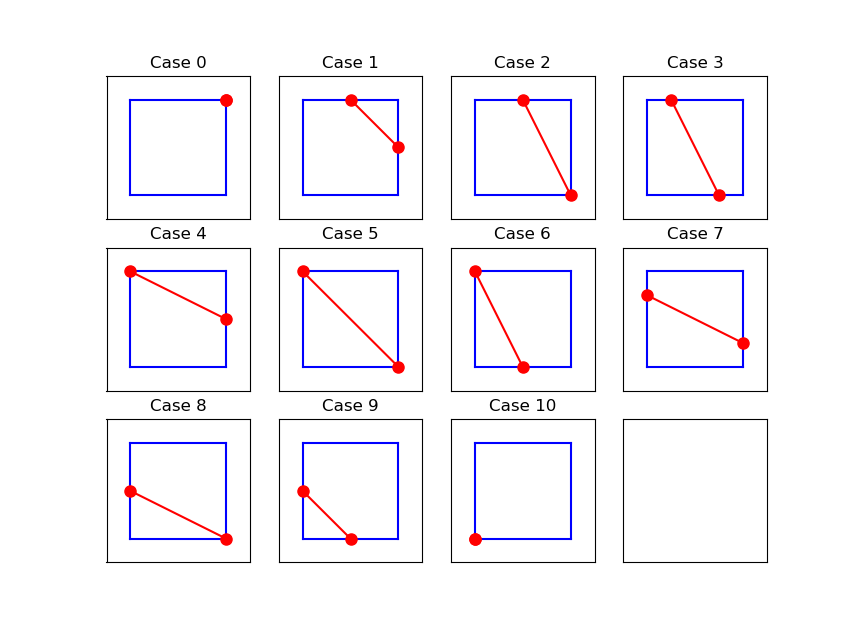
\includegraphics[scale=0.65]{integration_bounds_cases.png}
	\caption{Illustration of the various ways a line can cross a rectangular region assuming a negative-definite slope.}\label{fig:integration_bounds_cases}
\end{figure}



%%%%%%%%%%%%%%%%%%%%%%%%%%%%%%%%%%%%%%%%%%%%%%%%%%%%%%%%%%%%%%%%%%
\subsection{Meteoroid Projectile Mass Distribution}

From the MEM3 User Guide , we get the $g(m)$ flux of meteoroids larger than a limiting mass $m$, originally from \cite{grun1985collisional}. The Gr{\"u}n interplanetary flux equation is given by
\begin{equation}\label{eq:Grun_flux}
g(m) = (c_4m^{\gamma_4}+c_5)^{\gamma_5} + c_6(m + c_7m^{\gamma_6} + c_8m^{\gamma_7})^{\gamma_8} + c_9(m + c_{10}m^{\gamma_9})^{\gamma_{10}},
\end{equation}
where the constants are $c_4 = 2.2\times 10^3$, $c_5 = 15$, $c_6 = 1.3 \times 10^{-9}$, $c_7=10^{11}$, $c_8=10^{27}$, $c_9 = 1.3\times 10^{-16}$, $c_{10} = 10^6$; and the exponents are $\gamma_4 = 0.306$, $\gamma_5 = -4.38$, $\gamma_6 = 2$, $\gamma_7 = 4$, $\gamma_8 = -0.36$, and $\gamma_{10} = -0.85$. Eq.\ \ref{eq:Grun_flux} is applied to MEM's mass range and is shown in Figure \ref{fig:MEM_UG_Fig2.1_partile-mass-distribution}.

\begin{figure}[h!]
	\centering
	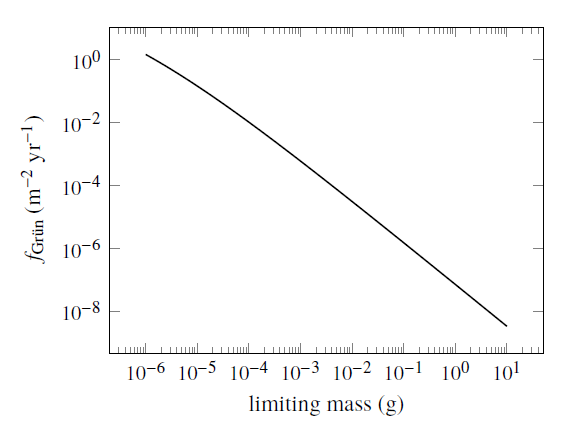
\includegraphics[scale=0.65]{MEM_UG_Fig2.1_partile-mass-distribution.PNG}
	\caption{The Gr{\"u}n interplanetary meteoroid flux as a function of limiting particle mass \citep[Figure 1]{moorhead2019nasa}.}\label{fig:MEM_UG_Fig2.1_partile-mass-distribution}
\end{figure}

The mass flux $dg(m)/dm$ and Eq.\ \ref{eq:HH11_mass-ejected1} should be integrated over the mass range $m_{min} = 10^{-6}$ g to $m_{max} = 10^1$~g in order to account for all impactor mass sizes, which we call $G_m$ given as
\begin{equation}\label{eq:Gm_integral}
G_m = \int_{m_{min}}^{m_{max}}dm\frac{dg(m)}{dm}m.
\end{equation}

The mass flux $dg(m)/dm$ can be fit to a double power law
\begin{equation}\label{eq:Grun_mass_flux}
\frac{dg(x)}{dx} = \frac{1}{ax^b+cx^d},
\end{equation}
where the fit parameters are shown in Figure \ref{fig:Fit-to-D_Grun}, using a log-log scale to capture the small and large masses correctly.

\begin{figure}[h!]
	\centering
	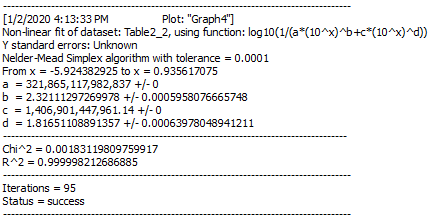
\includegraphics[scale=1]{Fit-to-D_Grun.PNG}
	\caption{Non-linear fit of Figure \ref{fig:MEM_UG_Fig2.1_partile-mass-distribution} with Eq.\ \ref{eq:Grun_mass_flux} in \textsf{SciDAVis}, giving the constants for $a$, $b$, $c$, and $d$.}\label{fig:Fit-to-D_Grun}
\end{figure}

To integrate Eq.\ \eqref{eq:Gm_integral}, we use the following solutions
\begin{align}\label{eq:Gm_int1}
\int dx\frac{x}{ax^b+cx^d} &= -\frac{1}{a(b-2)x^{b-2}} {}_2F_1\left[1, \frac{b-2}{b-d}; \frac{b-2}{b-d}+1; -\frac{c}{a}x^{d-b}\right],\\\label{eq:Gm_int2}
&= -\frac{1}{c(d-2)x^{d-2}} {}_2F_1\left[1, \frac{d-2}{d-b}; \frac{d-2}{d-b}+1; -\frac{a}{c}x^{b-d}\right],
\end{align}
where Eq.\ \ref{eq:Gm_int1} is more appropriate for small $x$ if $d-b > 0$ and Eq.\ \ref{eq:Gm_int2} is more appropriate for large $x$ if $d-b > 0$. If the sign of $d-b$ is flipped, then the small and large scale equations are swapped.


%%%%%%%%%%%%%%%%%%%%%%%%%%%%%%%%%%%%%%%%%%%%%%%%%%%%%%%%%%%%%%%%%%
\subsection{Meteoroid Projectile Density Distribution}

The meteoroid density has two components, a low and a high density contribution, as shown in Figure \ref{fig:MEM_UG_Fig2.5_density-distribution}. To take into account this particular distribution in computing the particle flux mass spectrum, we should integrate Figure \ref{fig:MEM_UG_Fig2.5_density-distribution} against Eq.\ \ref{eq:HH11_mass-ejected1}. Since the meteoroid density components can be written in terms of log-normal distributions
\begin{equation}\label{eq:log-normal_distribution}
F_\delta(x) = \frac{A}{\sigma\sqrt{2\pi}x}\exp\left[-\frac{(\ln x-\mu_\delta)^2}{2\sigma^2}\right],
\end{equation}
the integration entails computing the moments of a log-normal distribution. The $\alpha$-~moment is given by
\begin{equation}
F^\alpha_\delta(A,\mu_\delta,\sigma) = A\exp\left(\alpha\mu_\delta+\frac{1}{2}\alpha^2\sigma^2\right).
\end{equation}
Inserting these results into Eq.\ \ref{eq:HH11_mass-ejected1}, the functional form of the projectile density contribution can be written as
\begin{equation}
F_\delta = F^{3\nu-1}_\delta(A_{low}, \mu_{low},\sigma_{low}) + F^{3\nu-1}_\delta(A_{high}, \mu_{high},\sigma_{high}),
\end{equation}
where the fit parameters for the low and high density components are shown in Figures~\ref{fig:Fit-to-MEM_low_dens} and \ref{fig:Fit-to-MEM_high_dens}. Since the meteoroid density is given in units of \textit{fraction per 50 kg m$^{-3}$}, we need to divide the $A$ constants by 50 in order to give correct units.

\begin{figure}[h!]
	\centering
	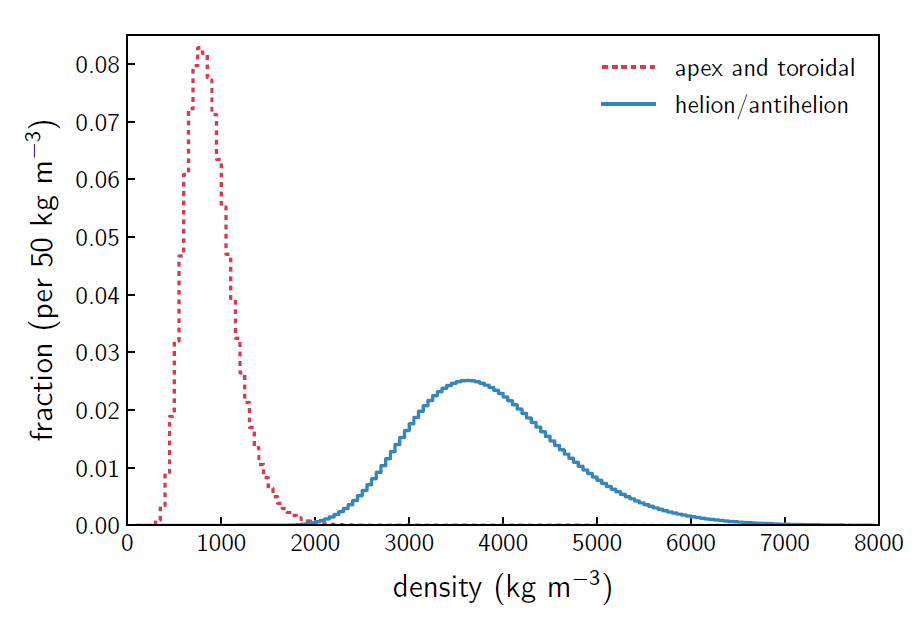
\includegraphics[scale=0.5]{MEM_UG_Fig2.5_density-distribution.PNG}
	\caption{Meteoroid density distribution according to the MEM3 User Guide. The apex and toroidal meteoroid sources constitute the low-density population, while the helion/antihelion source constitutes the high-density population. Each set of densities follows a log-normal distribution \citep[c.f. Figure 11,][]{moorhead2019nasa}.}\label{fig:MEM_UG_Fig2.5_density-distribution}
\end{figure}



\begin{figure}[h!]
	\centering
	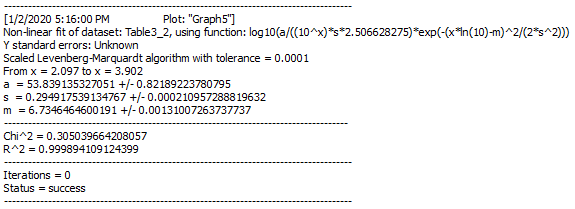
\includegraphics[scale=0.85]{Fit-to-MEM_low_dens.PNG}
	\caption{Non-linear fit of the low density profile in Figure \ref{fig:MEM_UG_Fig2.5_density-distribution} with Eq.\ \ref{eq:log-normal_distribution} in \textsf{SciDAVis}, giving the constants for $a\rightarrow A$, $s\rightarrow \sigma$, and $m\rightarrow \mu_\delta$.}\label{fig:Fit-to-MEM_low_dens}
\end{figure}

\begin{figure}[h!]
	\centering
	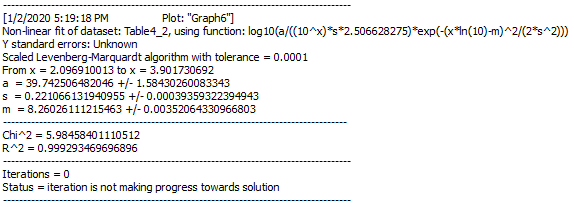
\includegraphics[scale=0.85]{Fit-to-MEM_high_dens.PNG}
	\caption{Non-linear fit of the high density profile in Figure \ref{fig:MEM_UG_Fig2.5_density-distribution} with Eq.\ \ref{eq:log-normal_distribution} in \textsf{SciDAVis}, giving the constants for $a\rightarrow A$, $s\rightarrow \sigma$, and $m\rightarrow \mu_\delta$.}\label{fig:Fit-to-MEM_high_dens}
\end{figure}

%%%%%%%%%%%%%%%%%%%%%%%%%%%%%%%%%%%%%%%%%%%%%%%%%%%%%%%%%%%%%%%%%%
\subsection{Meteoroid Projectile Speed and Angle Distribution}

MEM3 gives the incoming meteoroid flux (in units of \# per km$^2$ per year) in terms of the speed $U$ and both azimuth~$\theta$ and altitude $\phi$ angles for a location on the Moon. At the moment, since we are assuming azimuthally symmetric ejecta, we will sum over all $\theta$ azimuthal angles to simplify our calculation. In the future, we plan to incorporate azimuthal dependence for oblique impacts by including the azimuthal dependence of the ejecta blanket. The $\phi$ angle in MEM3 corresponds to our $\alpha$ angle, which is the impact angle with respect to the horizon. There are 36 $\phi$ bins\footnote{Half of the $\phi$ bins will always be zero, since they are below the horizon, so they can be ignored.} and 40 speed bins, after integrating over the 72 $\theta$ bins for each $\phi$ bin.


%%%%%%%%%%%%%%%%%%%%%%%%%%%%%%%%%%%%%%%%%%%%%%%%%%%%%%%%%%%%%%%%%%
\subsection{Secondary Ejecta Distance, Speed, \& Angle}

We would like to relate the distance from the meteorite impact to the secondary ejecta impact site by the secondary ejecta speed $v$ and angle $\gamma$ from zenith. If we assume the Moon is a perfect sphere with no atmosphere, we can calculate this distance by following the elliptical path the ejecta makes. The semi-major axis and eccentricity of the elliptical orbit are given by\footnote{See Eqs.\ 4.30 and 4.32 from http://www.braeunig.us/space/orbmech.htm.}
\begin{equation}\label{eq:a_of_v}
\frac{a}{r_m} = \frac{1}{2\left(1-\frac{v^2}{v_{esc}^2}\right)},
\end{equation}
where $r_m = 1737.1$ km is the radius of the Moon and $v_{esc} = 2.38$ km/s is the Moon's escape velocity, and
\begin{equation}\label{eq:e_of_v}
e = \sqrt{\left(\frac{2v^2}{v_{esc}^2}-1\right)^2\sin^2\gamma + \cos^2\gamma},
\end{equation}
where we employed the fact that the gravity of the Moon is $g = GM/r_m^2$ and the escape velocity is related by $v_{esc} = \sqrt{2gr_m}$. The third equation we need gives the location in the elliptical orbit by the angle $\beta$ from the perilune, the semi-major axis $a$, and the eccentricity $e$ by
\begin{equation}\label{eq:r_elliptical_orbit}
r = \frac{a(1-e^2)}{1+e\cos\beta}.
\end{equation}
Solving for $\cos\beta$ in Eq.\ \ref{eq:r_elliptical_orbit}, we have
\begin{equation}\label{eq:cos_elliptical_orbit}
\cos\beta = \frac{1}{e}\left(\frac{a(1-e^2)}{r}-1\right).
\end{equation}
In addition, we also need the equation for $\sin\beta$, which is given by (using a right triangle)
\begin{equation}
\sin\beta = \frac{1}{e}\sqrt{e^2-\left[\frac{a(1-e^2)}{r}-1\right]^2},
\end{equation}
so that $\tan\beta$ is
\begin{equation}\label{eq:tan_beta}
\tan\beta = \frac{\sqrt{e^2-\left[\frac{a(1-e^2)}{r}-1\right]^2}}{\frac{a(1-e^2)}{r}-1}.
\end{equation}

We found that the distance the secondary ejecta travels is given by the arc length of Moon the orbit travels greater than the radius of the Moon:
\begin{equation}\label{eq:D}
D = 2(\pi-\beta)r_m,
\end{equation}
or solving for the angle $\beta$,
\begin{equation}
\beta = \pi - \frac{D}{2r_m}.
\end{equation}
Using Eqs.\ \ref{eq:a_of_v} and \ref{eq:e_of_v}, we can write
\begin{equation}
\frac{a}{r_m}(1-e^2) = 2\frac{v^2}{v_{esc}^2}\sin^2\gamma,
\end{equation}
so Eq.\ \ref{eq:tan_beta} becomes \citep[c.f., Eq.\ (1) of][]{vickery1986size}
\begin{equation}\label{eq:ejecta_distance}
\tan\left(\frac{D}{2r_m}\right) = \frac{2\frac{v^2}{v_{esc}^2}\sin\gamma\cos\gamma}{1-2\frac{v^2}{v_{esc}^2}\sin^2\gamma} = \frac{\frac{v^2}{v_{esc}^2}\sin(2\gamma)}{\frac{v^2}{v_{esc}^2}[\cos(2\gamma)-1]+1}
=\frac{2\frac{v^2}{v_{esc}^2}\tan\gamma}{1+(1-2\frac{v^2}{v_{esc}^2})\tan^2\gamma}.
\end{equation}




%Therefore, we insert Eqs.\ \ref{eq:a_of_v}, \ref{eq:e_of_v}, and \ref{eq:D} into Eq.\ \ref{eq:cos_elliptical_orbit}, so that we now have the distance as a function of ejecta speed and angle from the zenith
%\begin{equation}\label{eq:ejecta_distance}
%\cos\left(\frac{D}{2r_m}\right) = \frac{1 - \frac{2v^2}{v_{esc}^2}\sin^2\gamma}{\sqrt{\left(1-\frac{2v^2}{v_{esc}^2}\right)^2\sin^2\gamma + \cos^2\gamma}}.
%\end{equation}
%Solving for the ejecta speed $v$, we can rewrite Eq.\ \ref{eq:ejecta_distance} in terms of the ejecta distance $D$ and zenith angle $\gamma$
%\begin{equation}
%\frac{v^2}{v_{esc}^2} = \frac{1}{2}\frac{\sin^2\left(\frac{D}{2r_m}\right)}{\cos^2\left(\frac{D}{2r_m}\right) - \sin^2\gamma}\left[\cot\left(\frac{D}{2r_m}\right)\cot\gamma - 1\right].
%\end{equation}
% Run plotSpeedAngleDistance.py
\begin{figure}[h!]
	\centering
	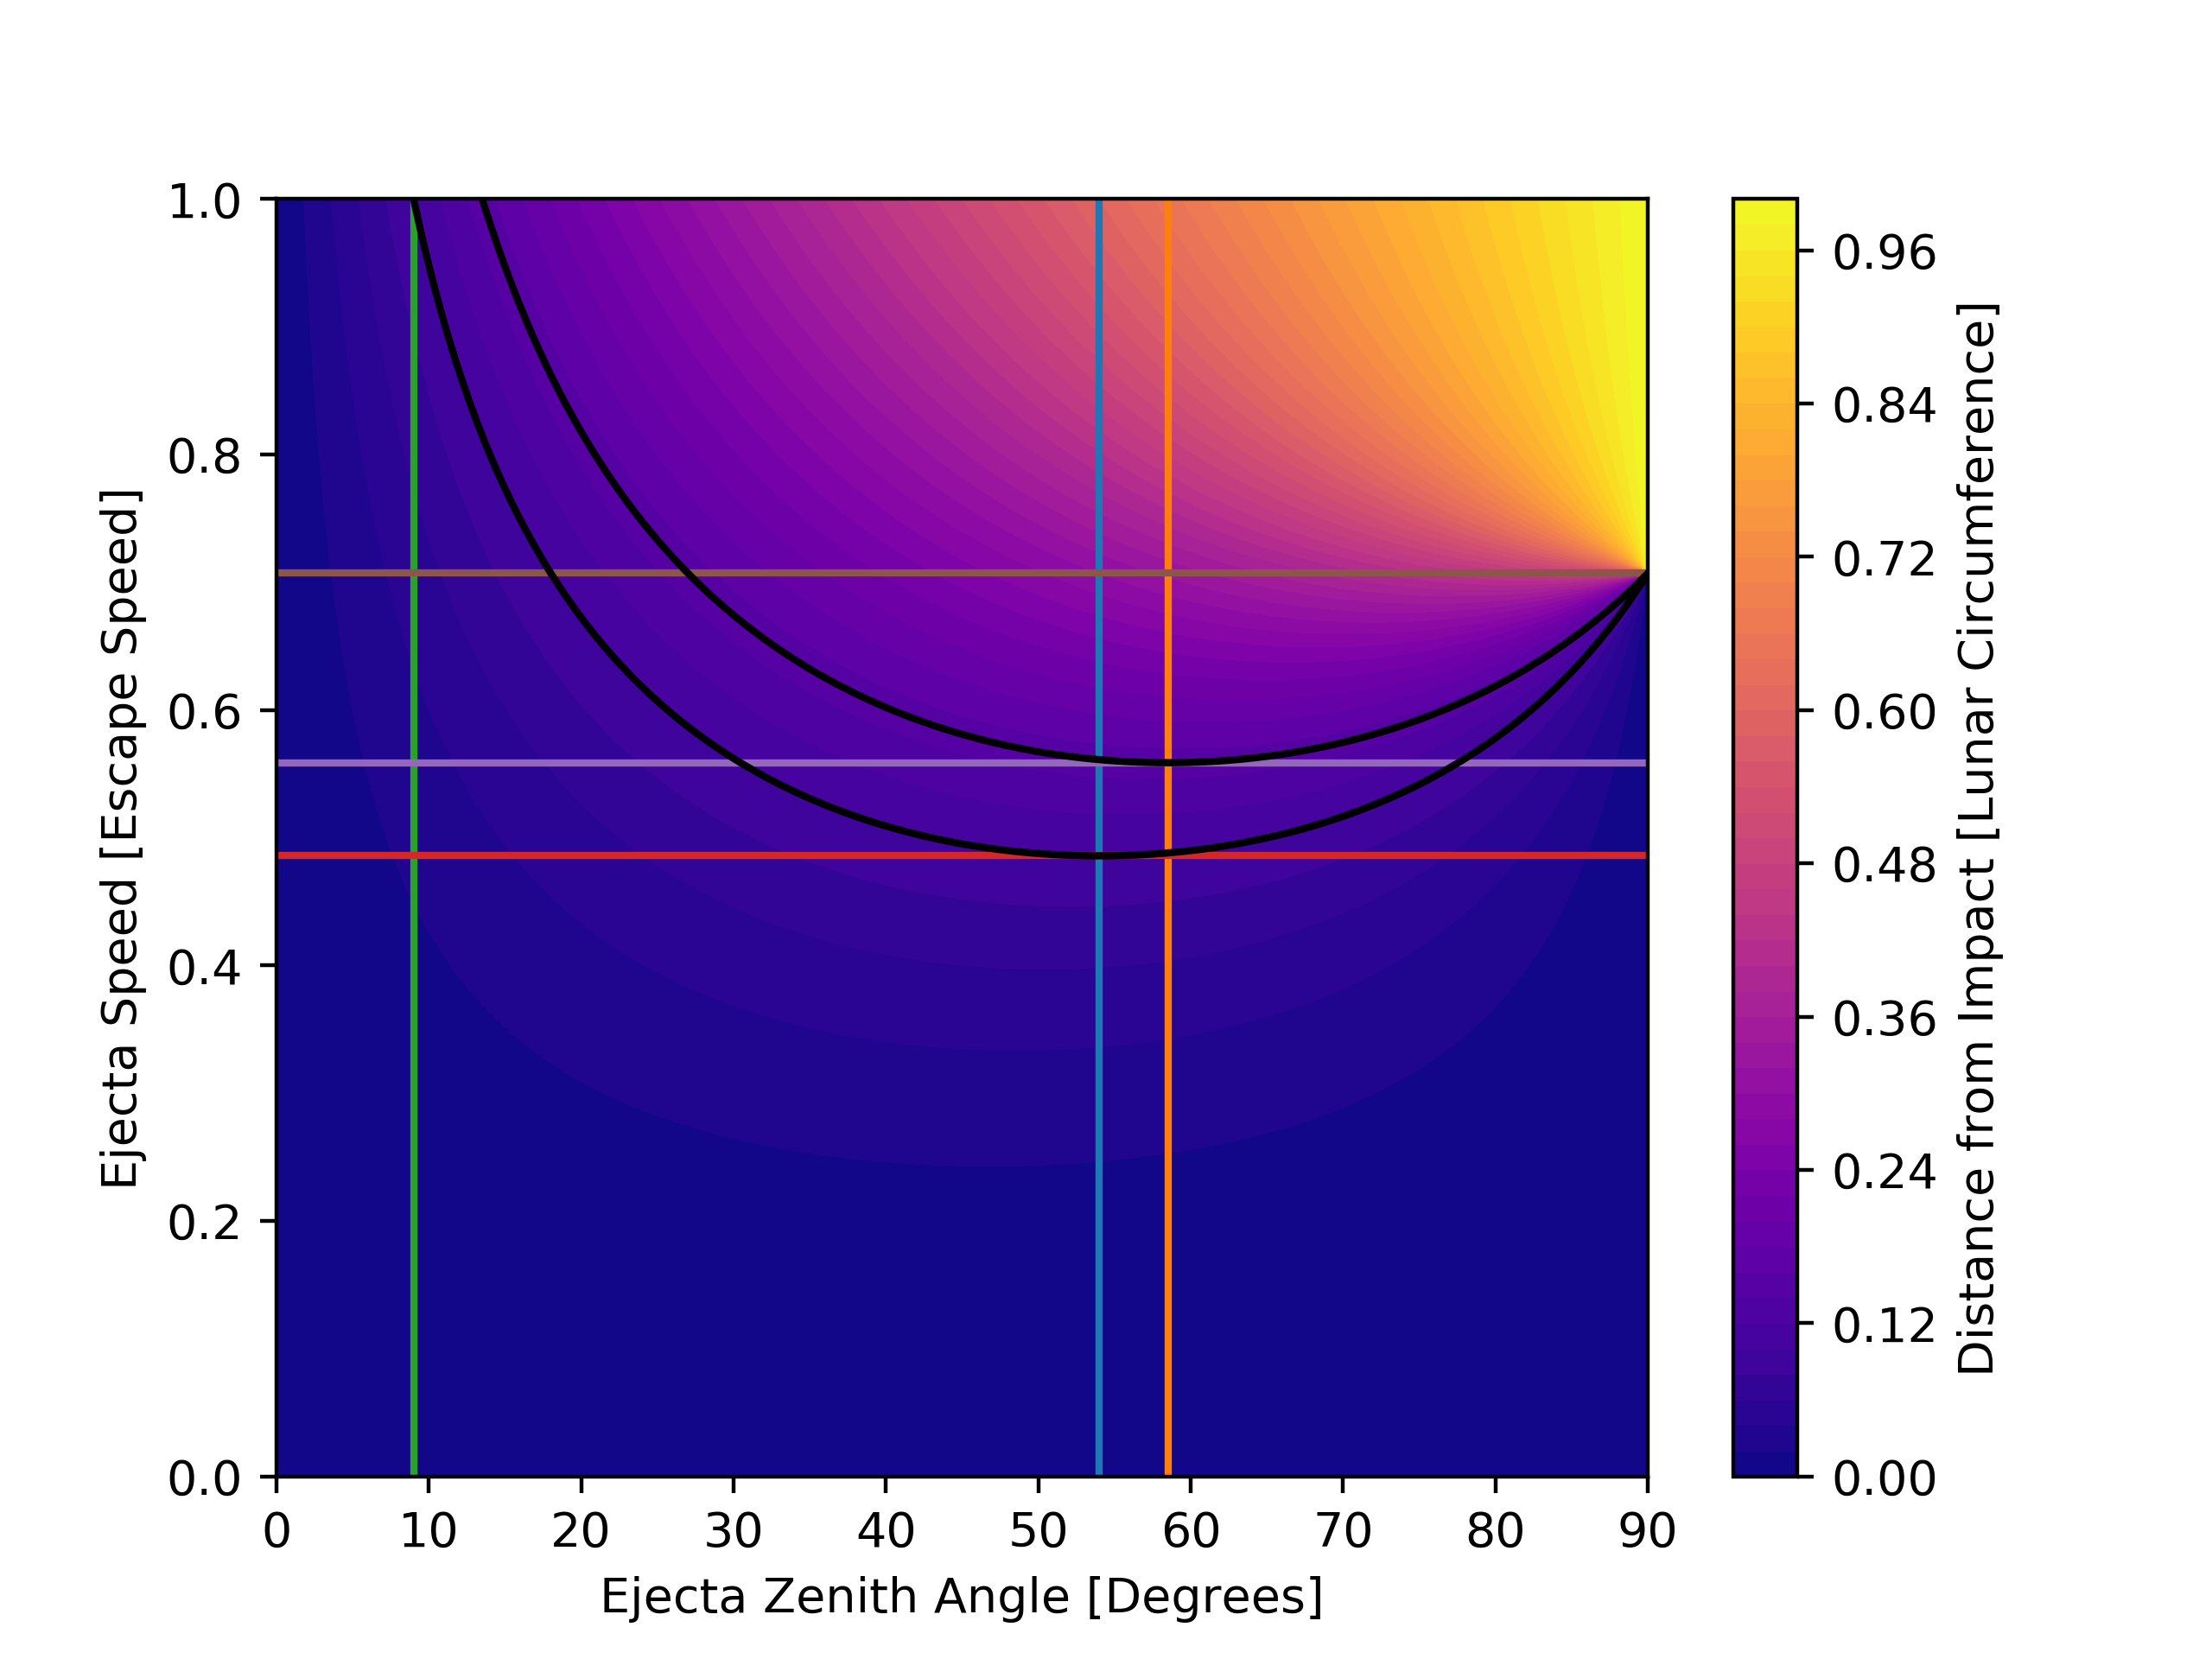
\includegraphics[scale=0.85]{../Distance_vs_EjectaSpeed_and_ZenithAngle.png}
	\caption{The color gradient shows the distance a projectile goes with a given ejected speed and zenith angle. The cyan dashed line gives the optimal angle for a given speed to reach the furthest distance, i.e., Eq.\ \eqref{eq:opt_angle}. The red dashed line shows for which pairs of speeds and zenith angles are required to hit the antipodal point. As an example, all ejecta with speed and angle pairs between the two black curves will reach a location between 0.05 and 0.06 lunar circumference units away, using Eq.~\eqref{eq:speed_asof_distance_angle}.}\label{fig:Distance_vs_EjectaSpeed_and_ZenithAngle}
\end{figure}



For $D \ll 2r_m$, the optimum angle that gives the smallest velocity needed is $45^\circ$. In other words, for a given velocity, the greatest distance is found by taking $\gamma = 45^\circ$. However, if the distance $D$ is roughly the same order as the diameter of the Moon $2r_m$, ($D > 0.01\times 2r_m$), then the optimal angle from zenith is greater than $45^\circ$, i.e.\ a shallower angle to the horizon. This is because at large velocities, the curvature of the Moon comes into play. For larger velocities, there are also angles $\gamma$ that cannot reach a distance $D$. Allowable angles (in radians) that can travel a distance $D$ are defined by
\begin{equation}
\gamma > \frac{D}{4r_m}.
\end{equation}
In other words, the maximum distance the ejecta can reach for a given angle is
\begin{equation}
D = 4\gamma r_m.
\end{equation}
For example, from this equation we can conclude that for $\gamma < 45^\circ$, the ejecta will not reach the antipodal point, see Figure \ref{fig:Distance_vs_EjectaSpeed_and_ZenithAngle}.


Solving for $v$ we have
%\begin{equation}
%\frac{v^2}{v_{esc}^2} = \left[1-\cos(2\gamma)+\sin(2\gamma)\cot\left(\frac{D}{2r_m}\right)\right]^{-1}
%\end{equation}
\begin{equation}\label{eq:speed_asof_distance_angle}
\frac{v}{v_{esc}} = \frac{+1}{\sqrt{\sin(2\gamma)\left(\cot\left(\frac{D}{2r_m}\right)+\tan\gamma\right)}}
= \frac{+1}{\sqrt{1+\sin(2\gamma)\cot\left(\frac{D}{2r_m}\right)-\cos(2\gamma)}}.
\end{equation}
We can also solve for the zenith angle $\gamma$, given by
\begin{equation}\label{eq:gammaVs_V_D}
\cot\gamma = x^2\cot\left(\frac{D}{2r_m}\right) \pm \sqrt{x^4\cot^2\left(\frac{D}{2r_m}\right) + (2x^2-1)},
\end{equation}
where $x = v/v_{esc}$. Solving for the discriminant, the minimum $x$ can be for a given distance $D$ is
\begin{equation}
x_{min}^2 = \tan^2\left(\frac{D}{2r_m}\right)\left[\csc\left(\frac{D}{2r_m}\right)-1\right].
\end{equation}
Plugging into Equation \ref{eq:gammaVs_V_D}, the optimal angle from zenith is given by
\begin{equation}\label{eq:opt_angle}
\cot\gamma_{opt} = \sec\left(\frac{D}{2r_m}\right) - \tan\left(\frac{D}{2r_m}\right).
\end{equation}
In terms of $x$, we have
\begin{equation}
\cos(2\gamma_{opt}) = \frac{x^2}{x^2-1}.
\end{equation}
Once $D > \pi r_m$, the optimal angle is $\gamma = 90^\circ$, i.e., parallel to the horizon. For small distances $D \ll 2r_m$, the optimal angle is $\gamma = 45^\circ$, as mentioned above.



\subsubsection{Coriolis Force}
The Coriolis force on secondary ejecta may also affect the ground path. To estimate the strength of the Coriolis force, the greatest speed due to the rotation of the Moon is at the equator, given by
\begin{equation}
v_c = \frac{2\pi r_m}{T} = \frac{2\pi * 1737.1 \text{ km}}{27.322 \text{ days}} = 4.62 \text{ m/s}.
\end{equation}
Therefore, we can ignore the Coriolis force if the ejecta speed $v$ is greater than roughly  $\sim10-15\times v_c$, or about $46$ m/s to $70$ m/s. This translates into ejecta distances less than $3$ km, which at those small distances the Coriolis force should not cause an effect anyways. So in general, we conclude that we can ignore the Coriolis force all together.

To quantify this conclusion, let us compute the Rossby number
\begin{equation}
R_o = \frac{v}{fL}.
\end{equation}

If we assume an ejecta angle of $45^\circ$, then plotting $D$ as a function of $v$ in Eq.\ \ref{eq:ejecta_distance} shows that $D \rightarrow L\sim v^2$. Taking our example above for $v=70$ m/s, $L = 3$ km, and $f = 2T$ to solve for $A$, we find that the Rossby number for secondary ejecta on the Moon is
\begin{equation}
R_o = \frac{A}{fv},
\end{equation}
where $A = 1.63$ m/s$^{2,}$\footnote{Curiously, this is basically the acceleration due to gravity on the Moon.}, $f = 5.328\times 10^{-6}$ rad/s, and $v$ is in units of m/s. In order to have $R_o\sim 1$ (small $R_o$ means the Coriolis forces cannot be ignored), we would need $v > 306$ km/s, which far exceeds the escape speed. The smallest $R_o$ can ever be is $R_o \sim 128$ when taking $v\to v_{esc}$. Therefore, we feel confident in our omission of the Coriolis force.

%%%%%%%%%%%%%%%%%%%%%%%%%%%%%%%%%%%%%%%%%%%%%%%%%%%%%%%%%%%%%%%%%%
\subsection{Distance and Bearing}\label{ssec:Distance_and_Bearing}
% see https://www.movable-type.co.uk/scripts/latlong.html

Given two latitude-longitude points on a sphere, $(\phi_1, \theta_1)$ and $(\phi_2, \theta_2)$, we can compute the distance and bearing following Chris Veness's webpage\footnote{\url{https://www.movable-type.co.uk/scripts/latlong.html}}.

The distance D is given by the equation
\begin{equation}\label{eq:shortdistance-between-latlon-points}
\tan\left(\frac{D}{2r_m}\right) = \sqrt{\frac{a}{1-a}},
\end{equation}
where $a$ is given by
\begin{equation}
a = \sin^2(\Delta\phi/2) + \cos\phi_1\cos\phi_2\sin^2(\Delta\lambda/2),
\end{equation}
for $\Delta\phi = \phi_2-\phi1$ and $\Delta\lambda = \lambda_2-\lambda_1$. Solving for the distance and simplifying, we have
\begin{equation}
D = 2r_m\arcsin(\sqrt{a}),
\end{equation}
or
\begin{equation}
D = 2r_m\arccos(\sqrt{1-a}).
\end{equation}

Other useful expressions involving trigonometric functions of $D/r_m$ are
\begin{align}
\sin(D/r_m) &= 2\sqrt{a(1-a)},\\
\cos(D/r_m) &= 1-2a,\\
\tan(D/r_m) &= \frac{2\sqrt{a(1-a)}}{1-2a}.
\end{align}

Eq.\ \eqref{eq:shortdistance-between-latlon-points} is the shortest distance between two coordinate points. For the long-distance, use
\begin{equation}
\tan\left(\pi-\frac{D}{2r_m}\right) = -\tan\left(\frac{D}{2r_m}\right) = \sqrt{\frac{a}{1-a}}.
\end{equation}

The initial bearing $\theta$ (from due East) is given by the following equation (assuming the short-distance):
\begin{equation}\label{eq:initial-bearing-shortdist}
\tan\theta_{i(1,2)} = \frac{\sin\Delta\lambda\cos\phi_2}{\cos\phi_1\sin\phi_2-\sin\phi_1\cos\phi_2\cos\Delta\lambda}.
\end{equation}
To find the final bearing (assuming the short-distance), swap $\phi_1\longleftrightarrow\phi_2$ and $\lambda_1\longleftrightarrow\lambda_2$ and reverse the angle such that
\begin{equation}\label{eq:final-bearing-shortdist}
\theta_{f(1,2)} = (\theta_{i(2,1)} + \pi)\mod 2\pi.
\end{equation}

In order to compute the initial and final bearing for the long-distance trajectory, add $\pi$ and then mod by $2\pi$ to Eqs.\ \eqref{eq:initial-bearing-shortdist} and \eqref{eq:final-bearing-shortdist}. In other words, swap initial and final bearings $\theta_{i(1,2)}\longleftrightarrow\theta_{f(1,2)}$.\\

We can also get the final latitude and longitude if we are given the distance $D$ and bearing $\theta$ from the starting location. The latitude and longitude are given by
\begin{align}
\phi_2 &= \arcsin\left[\sin\phi_1\cos(D/r_m) + \cos\phi_1\sin(D/r_m)\cos\theta\right], \\
\lambda_2 &= \lambda_1 + \arctan\left[\frac{\sin\theta\sin(D/r_m)\cos\phi_1}{\cos(D/r_m) - \sin\phi_1\sin\phi_2}\right].
\end{align}


%%%%%%%%%%%%%%%%%%%%%%%%%%%%%%%%%%%%%%%%%%%%%%%%%%%%%%%%%%%%%%%%%%
%%%%%%%%%%%%%%%%%%%%%%%%%%%%%%%%%%%%%%%%%%%%%%%%%%%%%%%%%%%%%%%%%%
\section{Meteoroid Ejecta Environment Output}

The goal of this chapter is to outline various outputs for the lunar meteoroid ejecta environment. For each section we will provide the techniques needed to evaluate the necessary integrals. Sections \ref{ssec:IntFlux_m_m} and \ref{ssec:IntFlux_Ec_Ec} will be for verification purposes, Section~\ref{ssec:IntFlux_d_d} will be for illustration, and Section \ref{ssec:IglooIntFlux_m} will be the engineering environment for the revision~H of DSNE, planed for the summer of 2020. The primary customer of the engineering environment will be the Appendix H contractors of the HLS (Human Landing System) Program.


%%%%%%%%%%%%%%%%%%%%%%%%%%%%%%%%%%%%%%%%%%%%%%%%%%%%%%%%%%%%%%%%%%
\subsection{Integral Flux ($>m$) vs.\ Particle Ejecta Mass}\label{ssec:IntFlux_m_m}

The integral flux of ejecta particles greater than mass $m$ as a function of particle ejecta mass $m$ for different ejecta speed ranges $v_{i}-v_{i+1}$ will aid in verifying against the NASA SP-8013 environment (Section \ref{sec:NASA SP-8013 Meteoroid Environment Model}) in addition to the work of Caleb Fassett (ref) and \cite{bjorkman2019astronaut}.


%%%%%%%%%%%%%%%%%%%%%%%%%%%%%%%%%%%%%%%%%%%%%%%%%%%%%%%%%%%%%%%%%%
\subsection{Integral Flux ($>E_{crit}$) vs.\ Critical Energy}\label{ssec:IntFlux_Ec_Ec}

The integral flux of ejecta particles great than critical energy $E_c$ as a function of critical energy $E_c$ for different speed ranges $v_{i}-v_{i+1}$ will be used to compare against \cite{bjorkman2019astronaut}.


%%%%%%%%%%%%%%%%%%%%%%%%%%%%%%%%%%%%%%%%%%%%%%%%%%%%%%%%%%%%%%%%%%
\subsection{Integral Flux ($>d$) vs.\ Particle Ejecta Size}\label{ssec:IntFlux_d_d}


%%%%%%%%%%%%%%%%%%%%%%%%%%%%%%%%%%%%%%%%%%%%%%%%%%%%%%%%%%%%%%%%%%
\subsection{Igloo Distribution of Integral Flux ($>m$)}\label{ssec:IglooIntFlux_m}





%%%%%%%%%%%%%%%%%%%%%%%%%%%%%%%%%%%%%%%%%%%%%%%%%%%%%%%%%%%%%%%%%%
\section{NASA SP-8013 Meteoroid Environment Model - 1969}\label{sec:NASA SP-8013 Meteoroid Environment Model}

The NASA SP-8013 Meteoroid Environment Model \citep{cour1969meteoroid}, is a document published in 1969 that describes the meteoroid and lunar ejecta environment of cometary origin with masses between $10^{-12}$ g and $1$ g. The flux-mass models and the associated density and velocity characteristics are for engineering applications in the design of space vehicles for near-Earth orbit, cis-lunar, lunar orbit, and lunar surface missions.

Our aim is to provide an updated specification to NASA SP-8013 for the lunar impact ejecta environment. Until the update is finished, DSNE points to Figure 10 (shown here in Figure \ref{fig:NASA-SP-8013-Fig10-flux-mass-distribution}) of \cite{cour1969meteoroid} for lunar ejecta. The results that follow from Sections \ref{sec:Spheral Based Lunar Ejecta Modeling} and \ref{sec:MEM3 Based Lunar Ejecta Modeling} will be verified against NASA SP-8013. We already anticipate that our new environments will be more benign (e.g., \cite[][pointing out that $50$ J is the critial energy]{bjorkman2019astronaut}), however to what degree from our analysis is yet to be determined. We also plan to provide output in terms of penetrating flux as a function of critical kinetic energy, as comparison to Figure 5 of \cite{bjorkman2019astronaut}, to aid in risk assessment of lunar impact ejecta.

\begin{figure}[h!]
	\centering
	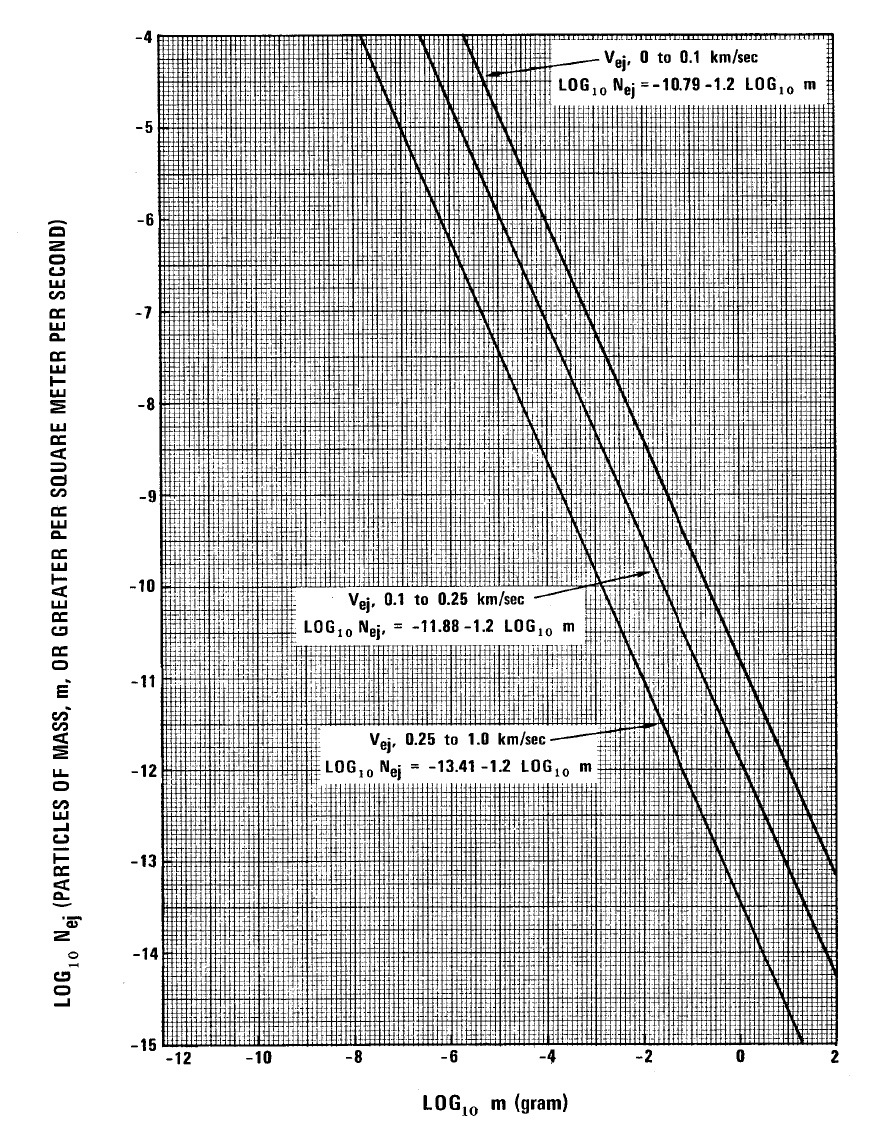
\includegraphics[scale=0.6]{NASA-SP-8013-Fig10-flux-mass-distribution.PNG}
	\caption{Average cumularive lunar ejecta flux-mass distribution for each of three ejecta velocity intervals \citep{cour1969meteoroid}.}\label{fig:NASA-SP-8013-Fig10-flux-mass-distribution}
\end{figure}


Our ultimate goal in providing an updated environment definition is to have an output in the same format as MEM 3's igloo files (see Section 3.4.4 of \cite{moorhead2019nasa}). This will allow for current analysis tools already familiar with MEM 3 to ingest our new environments without modification to those tools. 


%%%%%%%%%%%%%%%%%%%%%%%%%%%%%%%%%%%%%%%%%%%%%%%%%%%%%%%%%%%%%%%%%%
%%%%%%%%%%%%%%%%%%%%%%%%%%%%%%%%%%%%%%%%%%%%%%%%%%%%%%%%%%%%%%%%%%
%\section{References}
\cleardoublepage
\phantomsection
\addcontentsline{toc}{section}{References}
\bibliographystyle{agu}
\bibliography{report}

\end{document}